\renewcommand{\typeRubriek}{loep}		

%%%%%%%%%%%%%%%%%%%%%%%%%%%%%
% informatie voor de auteur %
%%%%%%%%%%%%%%%%%%%%%%%%%%%%%
% de soorten titels opmaakmogelijkheden die de auteur kan gebruiken:
% section
% section*, betekent dat er geen nummer bij gezet wordt
% subsection
% tussentitel
% citaat
% opsomming
% nummering
% bronnen
% kader
% stellingkader (genummerd)
% stellingkadertwee (niet genummerd)
% kleurkader
% werktekst



% twee parameters voor nieuwe rubriek: titel en auteur (die mogen ook leeggelaten worden o.a. voor redactioneel)
\startNieuweRubriek{Lessen uit afstandsonderwijs}{Gerd Hautekiet, Els Van Emelen\\en Gilberte Verbeeck}

\startcontents[mainsections]		      % om opsomming in inhoudstafel enkel tot loep te beperken
\begin{multicols}{2}                      
\inhoudstafelLoep		                  % om inhoudstafel in te voegen



%%%%%%%%%%%%%%%%%%%%%%%%%%%%%%%%%%%%%%%%%%%%%%%%%%%%%%%%%%%%%%%%
%%%%%%%%%%%           START VAN DE TEKST               %%%%%%%%%%
%%%%%%%%%%%%%%%%%%%%%%%%%%%%%%%%%%%%%%%%%%%%%%%%%%%%%%%%%%%%%%%%

\section{Inleiding}

Op het moment dat dit nummer verschijnt, zal COVID-19 ons leven al bijna een jaar tekenen. Sinds het voorjaar van 2020 domineert het onderwerp de binnenlandse en buitenlandse pers. De kranten, het televisienieuws maar ook de vakliteratuur bespreken dit onderwerp zeer uitgebreid. Daardoor lezen we vaak hetzelfde, overgoten met een andere saus. Ook in Uitwiskeling ontsnap je hier niet aan.

Toen we voor deze loep ideeën sprokkelden, voelden we zelf verzadiging bij de aanhoudende stroom van crisisberichten. Daarom besloten we het over een andere boeg te gooien en er vanuit een ander standpunt naar te kijken: we vatten de lockdown op als `een (lange) ervaring die helpt om ons onderwijs te verbeteren'. Het was een eenzame periode waarin we leerlingen vanachter een computerscherm zo goed mogelijk ondersteunden. Dat was geen sinecure. Helemaal buiten onze comfortzone experimenteerden we. We gaven online lessen, maakten filmpjes, bedachten stappenplannen, corrigeerden pdf-bestanden en foto’s met of zonder smartpen… Een verwarrende tijd waarin we gedwongen werden om in sneltempo vele nieuwe dingen te leren. Weinig leraren wilden naar deze periode van afzondering terug. 

Tijdens de hete zomer van 2020 namen we tijd voor contemplatie en reflectie. Vanop een afstand keken we kritisch terug. Nieuwe dingen uitproberen zorgt immers voor nieuwe inzichten. Deze loep is een poging om een aantal van deze inzichten enerzijds scherp en anderzijds concreet te maken. We zoeken uit hoe `wat we toen leerden' ons onderwijs kan versterken. Oogsten heet dat.

Deze loep is zeker geen pleidooi voor digitaal leren of afstandsonderwijs. Integendeel! Zoals je in het vorige redactioneel al kon lezen, kiezen we vol overtuiging voor nabij en interactief onderwijs. Echter, we zijn niet vies van digitale hulpmiddelen die dit onderwijs kunnen versterken of onszelf kunnen ondersteunen.

De loep bevat vier grote onderdelen. Eerst lichten we enkele inzichten toe die de coronacrisis scherper maakte. In de tweede paragraaf lees je over ervaringen die we niet zonder meer los willen laten. We vragen ons af hoe ze ons onderwijs kunnen versterken. Misschien inspireren ze. De derde paragraaf bevat een aantal bronnen die we tijdens de coronacrisis ontdekten en die we waardevol vinden. En tot slot eindigen we met een kleine `toolkit voor noodgevallen' mochten we opnieuw in dit soort situatie belanden. 

Ondertussen steeg tijdens de herfst het aantal besmettingen opnieuw exponentieel en konden we een tweede lockdown niet langer vermijden. Tijdens de redactievergaderingen - eerst met afstand, later online - wisselden we telkens nieuwe ideeën en ervaringen uit. We schreven daarom ook soms in de ik-vorm en soms in de we-vorm, een bundeling van ervaringen van de hele redactie. 
\end{multicols}

\begin{figure}[H]
\begin{center}

\includegraphics[width=12cm]{tekeningenKurt/uw november 2020 hangmat.jpg}
\end{center}
\end{figure}
%\vspace{0.5cm}

%\subsection{Typ hier de deelparagraaftitel}
%Typ hier je tekst
%\tussentitel{Typ hier de tussentitel}

\begin{multicols}{2}
\section{Aangescherpte inzichten}

Tijdens de eerste lockdown zorgden we op een andere manier voor onderwijs. Doordat deze ervaringen zo anders waren (schuin gedrukt in de onderstaande tekst), liet het ons stilstaan bij wat we misten, wat we belangrijk vinden in onze lessen, wat nodig is voor goed onderwijs en wat meer aandacht mag krijgen.

\tussentitel{De kracht van een goed (onderwijsleer)gesprek}
\emph{Om de voorkennis van de leerlingen op te roepen, start ik mijn digitale les met een vraag: `Welke verschillende functies hebben we tot hiertoe al behandeld?' Er valt een stilte. Oogcontact is er niet. Leerlingen kijken naar beneden of naast me door, schrijven iets op een blad. Lichaamstaal die ik niet kan inschatten en waar ik niet op kan reageren.   Sommige leerlingen vind ik alleen maar in de deelnemerslijst. Hun camera staat uit. Niemand voelt zich aangesproken. Het wordt gênant... Ik durf niet langer wachten en beantwoord mijn eigen vraag... }

Het onderwijsleergesprek waar slechts één iemand spreekt, is een monoloog. Soms is een monoloog waardevol. Een goed opgebouwde redenering biedt immers structuur en helderheid. Met een onderwijsleergesprek beoog je iets anders. De kracht van zo een gesprek zit in de interactie. Wanneer een leerling op een vraag antwoordt, maakt hij duidelijk wat hij al begrijpt en waar hij de bal nog misslaat. De vraag die hij stelt, toont hoe hij meedenkt en waar hij vastloopt in de redenering. De lichaamstaal die leerlingen gebruiken, zoals een opgetrokken wenkbrauw of een frons, werkt drempelverlagend. Voor de leraar is een klein gebaar vaak al genoeg om te weten wat er aan de hand is. Daarnaast kan hij met zijn lichaam ook sturen. Even de hand opsteken om aan te geven dat leerlingen niet door de klas mogen roepen. Met humor en `toneelspel' zorgt hij voor een sfeer waar geleerd kan worden: veilig en boeiend.

\tussentitel{De rijkheid van de leerlingen}
\emph{Zuchtend kijk ik naar mijn scherm. Ik heb al drie kwartier filmmateriaal opgenomen en vraag me af hoe ik mijn eigen monoloog kan doorbreken. Ik wil de leerlingen meer bij het onderwijsgebeuren betrekken. In de klas doe ik dat door hen geregeld een opgave aan bord te laten uitleggen. Dan wordt snel zichtbaar wat ze al kunnen en wat nog niet. Dat kan nu niet. Ik heb geen bord en geen leerlingen. Ten einde raad post ik in het klas-whatsapp-groepje de opdracht: `Film jezelf terwijl je luidop een vraagstuk oplost.' Nadat de eerste leerling de spits heeft afgebeten, druppelen de filmpjes binnen. Ze doen hun best, dat zie ik. Wat bij de ene goed gaat, loopt bij de andere nog fout en omgekeerd. Ik kan elke leerling aangepaste feedback geven. En op het einde van de rit zijn alle belangrijke dingen aan bod gekomen.}

Werken met leerlingen brengt rijkdom in het leerproces. De klasgroep mag niet te klein zijn, anders krijg je niet genoeg diversiteit. Maar ook niet te groot, want dan verlies je het overzicht. De rijkheid zit in wat ze inbrengen maar ook wat ze van elkaar oppikken. Daarnaast biedt een groep ook de mogelijkheid om even weg te zakken. Het is geruststellend om niet altijd in de picture te staan, te mogen afwachten wat er gebeurt en dan terug aan te pikken. 

\tussentitel{De leraar aan het roer}

\emph{Met een aantal wiskundecollega's kijk ik naar een promotiefilmpje van Snappet. Snappet is een online platform dat elke leerling een aangepast aanbod geeft. Voor een bepaald onderwerp selecteert het programma, op basis van de juist opgeloste opgaven, een nieuwe set die past bij het niveau van de leerling. Je hebt er als leraar geen werk aan. Op het eerste gezicht klinkt het geweldig, zeker in deze coronatijden waar het leerproces digitaal aansturen en afchecken een grote hulp zou zijn. }

Maar als we het van dichterbij bekijken, hebben we serieuze bedenkingen. De leraar heeft niet langer de regie in handen. Dat zie je op verschillende vlakken. 

De les start met een filmpje dat de leerstof toelicht. Handig in coronatijden. Er bestaan natuurlijk goede filmpjes. Toch leggen de meeste filmpjes de leerstof op een andere manier uit dan ikzelf zou doen. Vaak ligt de focus vooral op `Hoe los ik dit goed op?' eerder dan op `En waarom klopt dit?' Een belangrijk nuanceverschil.

Daarnaast bepaalt het programma welke opdrachten een leerling krijgt. Dat lijkt comfortabel maar je hebt geen overzicht welke opgaven in het pakket zitten en of dit ook de opgaven zijn waarvan jij het belangrijk vindt dat leerlingen erover nadenken.

Tot slot, leerlingen krijgen onmiddellijk feedback wanneer ze een oefening oplossen. Dat klinkt goed. Maar in concreto betekent dit dat ze een rode of een groene ampersand op hun scherm te zien krijgen. Wiskunde wordt als het ware herleid tot het oplossen van een quiz waar de antwoorden goed of fout zijn. Er is geen nuance, geen waardering voor een mooie oplossing, geen discussie over het antwoord.

Bij het digitaliseren van de leeromgeving loop je het gevaar dat je onderwijs aansluit bij een onderwijstheorie, dat het in onderwijs enkel om leerprestaties zou gaan. Kiezen voor een leraar die werelden voor je opent, gaat uit van een andere visie op onderwijs. Daar is een goede leraar een gids, een liefhebber van zijn vak die de schoonheid daarvan kan en wil laten zien.


\tussentitel{Voor-leren en na-leren ondersteunen}

\emph{Na de paasvakantie mochten we `preteachen'. Dit als voorbereiding voor de heropstart van de scholen later in het schooljaar. Het woord werd in de media erg populair. Het gebruik ervan verwarde mij vooral. Ik kende deze werkwijze vanuit het remediërend leren waar de betekenis anders wordt ingevuld.}

Wikipedia omschrijft `preteaching' als een activiteit je die doet \emph{voorafgaand} aan de klassikale instructie. Samen met leerlingen die moeite hebben met het verwerven van de leerstof, zoom je op voorhand in op de nieuwe leerstof. Daardoor horen deze leerlingen de uitleg tweemaal, hetgeen een positief effect heeft op de leeropbrengsten. Het concept van preteaching kan daaraan een waardevolle bijdrage leveren. `Voor-leren' zou de Nederlandse vertaling kunnen zijn. 

De term kreeg in tijden van corona een nieuwe (foute?) lading. Je kon immers niet van voor-leren spreken omdat er daarna `in real life' niet dezelfde les volgde. Heel wat klassen hadden verderop in het schooljaar weinig of zelfs geen offline lessen meer. 

Naast preteachen is er ook `flipping the classroom'. Hierbij laat je de leerlingen op voorhand de theorie, bv. onder de vorm van een instructiefilmpje, doornemen. In de les gebruik je deze kennis om toepassingen of oefeningen te maken. Zo wissel je gezamenlijke luister-tijd in voor gezamenlijke oefen-tijd.

Beide concepten zijn boeiend. Naast voor-leren zou je ook kunnen nadenken over na-leren. Tijdens de lockdown nam ik heel wat instructiefilmpjes op. Die kan ik nu na de les aanbieden. Leerlingen die de uitleg graag nog een tweede keer horen, kunnen thuis rustig nog een keer naar het filmpje kijken. 

\tussentitel{De waarde van het zoeken}

\emph{Begin september sta ik opnieuw voor een volle klas. Het voelt raar. De banken staan meer dan een meter uit elkaar en ik heb de opdracht gekregen om vooraan te blijven. Moeilijk. Het valt me op hoe sommige gedragsgewoonten snel ingeburgerd raken: handen ontsmetten, mondmaskers gebruiken, even online overleggen. Ook op vlak van leren zijn er dingen veranderd. Leerlingen hebben meer moeite om zich lang te concentreren, ze zijn zelfstandiger en een digitale opdracht gaat sneller, maar hun wiskundige vaardigheden zijn minder geoefend. Plots stelt een leerling de vraag of ik hen de oplossingen van de opgaven nog bezorg. Ik denk na, voel twijfel en zeg nee...}

Tijdens de lockdown zochten we hoe we konden omgaan met het eindeloze verbeterwerk. Leerlingen zelf hun opgaven laten corrigeren door te vergelijken met een sleutel was een goed hulpmiddel. Nu we opnieuw samen in de klas aan het werk gaan, denk ik na over de voor- en nadelen van een sleutel. Ik begrijp het verlangen van leerlingen naar zekerheid. Is deze oplossing juist? Moet het zo? Toch wil ik de sleutel niet zonder meer geven. Leerlingen die moeite met bepaalde opgaven hebben zeggen vaak: `Ik kan het niet zelf vinden maar als ik de oplossing zie, begrijp ik het altijd.' Er is meer nodig om iets te kunnen dan voldoende uitgewerkte voorbeelden krijgen.

Zoeken, proberen, twijfelen is waardevol. Je leert bij door een stukje van de oplossing te vinden en die daarna bij te sturen, door overleg met medeleerlingen, door samen te denken, door een tip te krijgen waarmee je verder kunt zoeken. Al deze elementen neem je weg op het moment dat je een sleutel geeft. Dit soort zoeken is nodig voor de ontwikkeling van het probleemoplossend denken of voor het ontwikkelen van zoekstrategieën, vaardigheden die intrinsiek met wiskunde verbonden zijn. 

\section{Onderwijs versterken}
\subsection{Filmmateriaal} 
\emph{Waar is de tijd dat
ik mijn examens met de hand schreef? Het lijkt ontzettend ver weg. Tegenwoordig schrijf ik veel minder en bijgevolg hoe langer hoe lelijker. Mijn slimme telefoon is mijn agenda, mijn geheugensteuntjesopslag, mijn camera, mijn betaalmiddel, een didactisch middel en zo veel meer. Een foto van een oefening is in een handomdraai genomen en een filmpje met wat uitleg gaat me vlotter af dan schrijven.}

Werken met foto's en filmpjes behoorde al voor een stukje tot onze onderwijspraktijk. De beperkte kennis die we hadden, bleek goed bruikbaar tijdens de coronacrisis. Meer nog, we leerden bij en het werd een belangrijk onderdeel van het online lesgeven. Nu we erop terugblikken, merken we dat de filmpjes die de leerlingen en wijzelf maakten, een blijvende waarde kunnen hebben in onze onderwijspraktijk.

\tussentitel{Leerlingen maken filmpjes}
Mijn leerlingen maakten hoofdzakelijk drie soorten filmpjes. Ze trokken een foto van een theoretisch stukje of een oefening.  Vervolgens maakten ze daarbij een filmpje waarin ze één of meerdere vragen stelden die ze hadden. In een tweede soort filmpje namen ze zichzelf op terwijl ze luidop een vraagstuk oplosten. Voor de derde soort schreven ze eerst een oefening uit, om vervolgens tijdens een opname de oefening en dus hun redenering uit te leggen.
We kregen uiteraard filmpjes binnen van heel uiteenlopende inhoudelijke kwaliteit. Dat is op zich niet verrassend. Het was voor veel leerlingen de eerste keer dat ze zoiets maakten. 

\tussentitel{Leraren maken filmpjes}
Ook leraren maken verschillende soorten filmmateriaal. We geven een overzicht. 

Een eerste type vertrekt vanuit het materiaal dat de leerling inleverde. De leerling stuurt een foto met een oefening. De leraar geeft hierop feedback via een filmpje, eventueel ondersteund door geschreven commentaar. 

Voor een tweede vorm van filmmateriaal vertrekt de leraar vanuit de oplossingensleutel die een handboek aanbiedt. Bij de meeste handboeken kun je tegenwoordig al dan niet uitgebreide handleidingen met antwoordmodellen aanschaffen. Het gebeurt dat we het niet (helemaal) eens zijn met het antwoordmodel van het boek of dat we die te beperkt vinden. In een filmpje kunnen we extra uitleg of duiding geven bij het antwoordmodel zonder dat we de hele oefening opnieuw moeten uitschrijven. Soms bieden we liever een alternatieve oplossing aan. Ook hier kan gesproken tekst in een filmpje aanvulling bieden. De leraar maakt een verbetersleutel en spreekt hierbij een filmpje in.

Een derde type vinden we terug wanneer we onszelf filmden wanneer we instructie gaven. Er zijn verschillende varianten. 

We maakten filmpjes bij een powerpoint die langzaam een uitleg opbouwt of filmpjes terwijl we zelf een oefening oplosten. Het mooie hierbij is dat je de opbouw geleidelijk ziet verschijnen en de leerling tijd krijgt om mee te redeneren.  

Daarnaast trokken verschillende onder ons naar de klas en stelden de camera op tegenover het bord. We doceerden een stukje theorie of een oefening en gaven les aan een lege klas voor het oog van de camera. 

We maakten ook filmpjes die we gebruikten in onze online lessen. Sommige zaken kunnen niet of niet eenvoudig op de computer gemaakt worden, denk bv. aan een kansboom. Door de kansboom te tekenen op een blad papier en dit te filmen, kon je dit filmpje gebruiken tijdens de online les. Voordeel is dat je het kunt stopzetten, terugspoelen enz... terwijl je uitleg geeft.  

Een laatste variant is het opnemen van de online lessen. Deze opnames behoren tot het filmmateriaal dat we ondertussen ter beschikking hebben. We hebben de tijd nog niet genomen om het terug te bekijken. Dat is zeker relevant naarmate we dichter bij maart 2021 komen of als we een onderwerp uit de opnames terug in de klas gaan brengen. 

\tussentitel{Onderwijs versterken met filmmateriaal}

De filmpjes die leerlingen instuurden, hebben als meerwaarde dat we iedereen aan het woord kunnen horen. Ook leerlingen die in de klas weinig inbrengen, krijgen spreekruimte in zo'n filmpje. Het is een werkvorm waarmee we de wiskundige taalvaardigheid van leerlingen kunnen verbeteren. Dat maakt het de moeite om dit soort activiteit als `een blijver' te bestempelen. 

Daarnaast vormen deze filmpjes een schat aan materiaal om een inhoud in het midden te leggen ter bespreking. Je kunt er nieuwe opdrachten mee opstellen door bij een filmpje vragen te stellen, feedback te geven zodat ze hun oplossing kunnen bijsturen... Daarbij zoomen we zowel in op wiskundige inhoud als wiskundige verwoording.

Ook in niet-coronatijden dienen leerlingen oefeningen in ter correctie of gebruik je een verbetersleutel van de handleiding. We merkten dat het opnemen van een filmpje een veel snellere en meer toegankelijke manier is om feedback te geven dan het uitschrijven van die feedback. Al haalt dit het natuurlijk niet bij een echt gesprek over deze materie. 

Verder kunnen we filmpjes of stukken filmpjes die we maakten, hergebruiken voor `preteaching' of `flipping the classroom'. Sommige leerlingen gaven expliciet aan dat ze het heel fijn vonden om de les terug te kunnen bekijken en een filmpje terug te kunnen spoelen op punten waar ze het niet goed begrepen. Op deze manier kunnen we trage leerders extra materiaal geven voor of na de les. Leerlingen die afwezig waren of remediëring nodig hebben, kunnen zichzelf bijwerken op basis van het opgenomen materiaal.

Een originele manier om dit materiaal te gebruiken hoorden we tijdens de redactievergadering. Een collega had bij het lesgeven met een mondmasker 's avonds veel last van zijn stem. Hij gebruikte de opgenomen filmpjes tijdens een offline les om zijn stem te sparen. 



\end{multicols}
%\vspace{0.5cm}
\begin{figure}[H]
\begin{center}
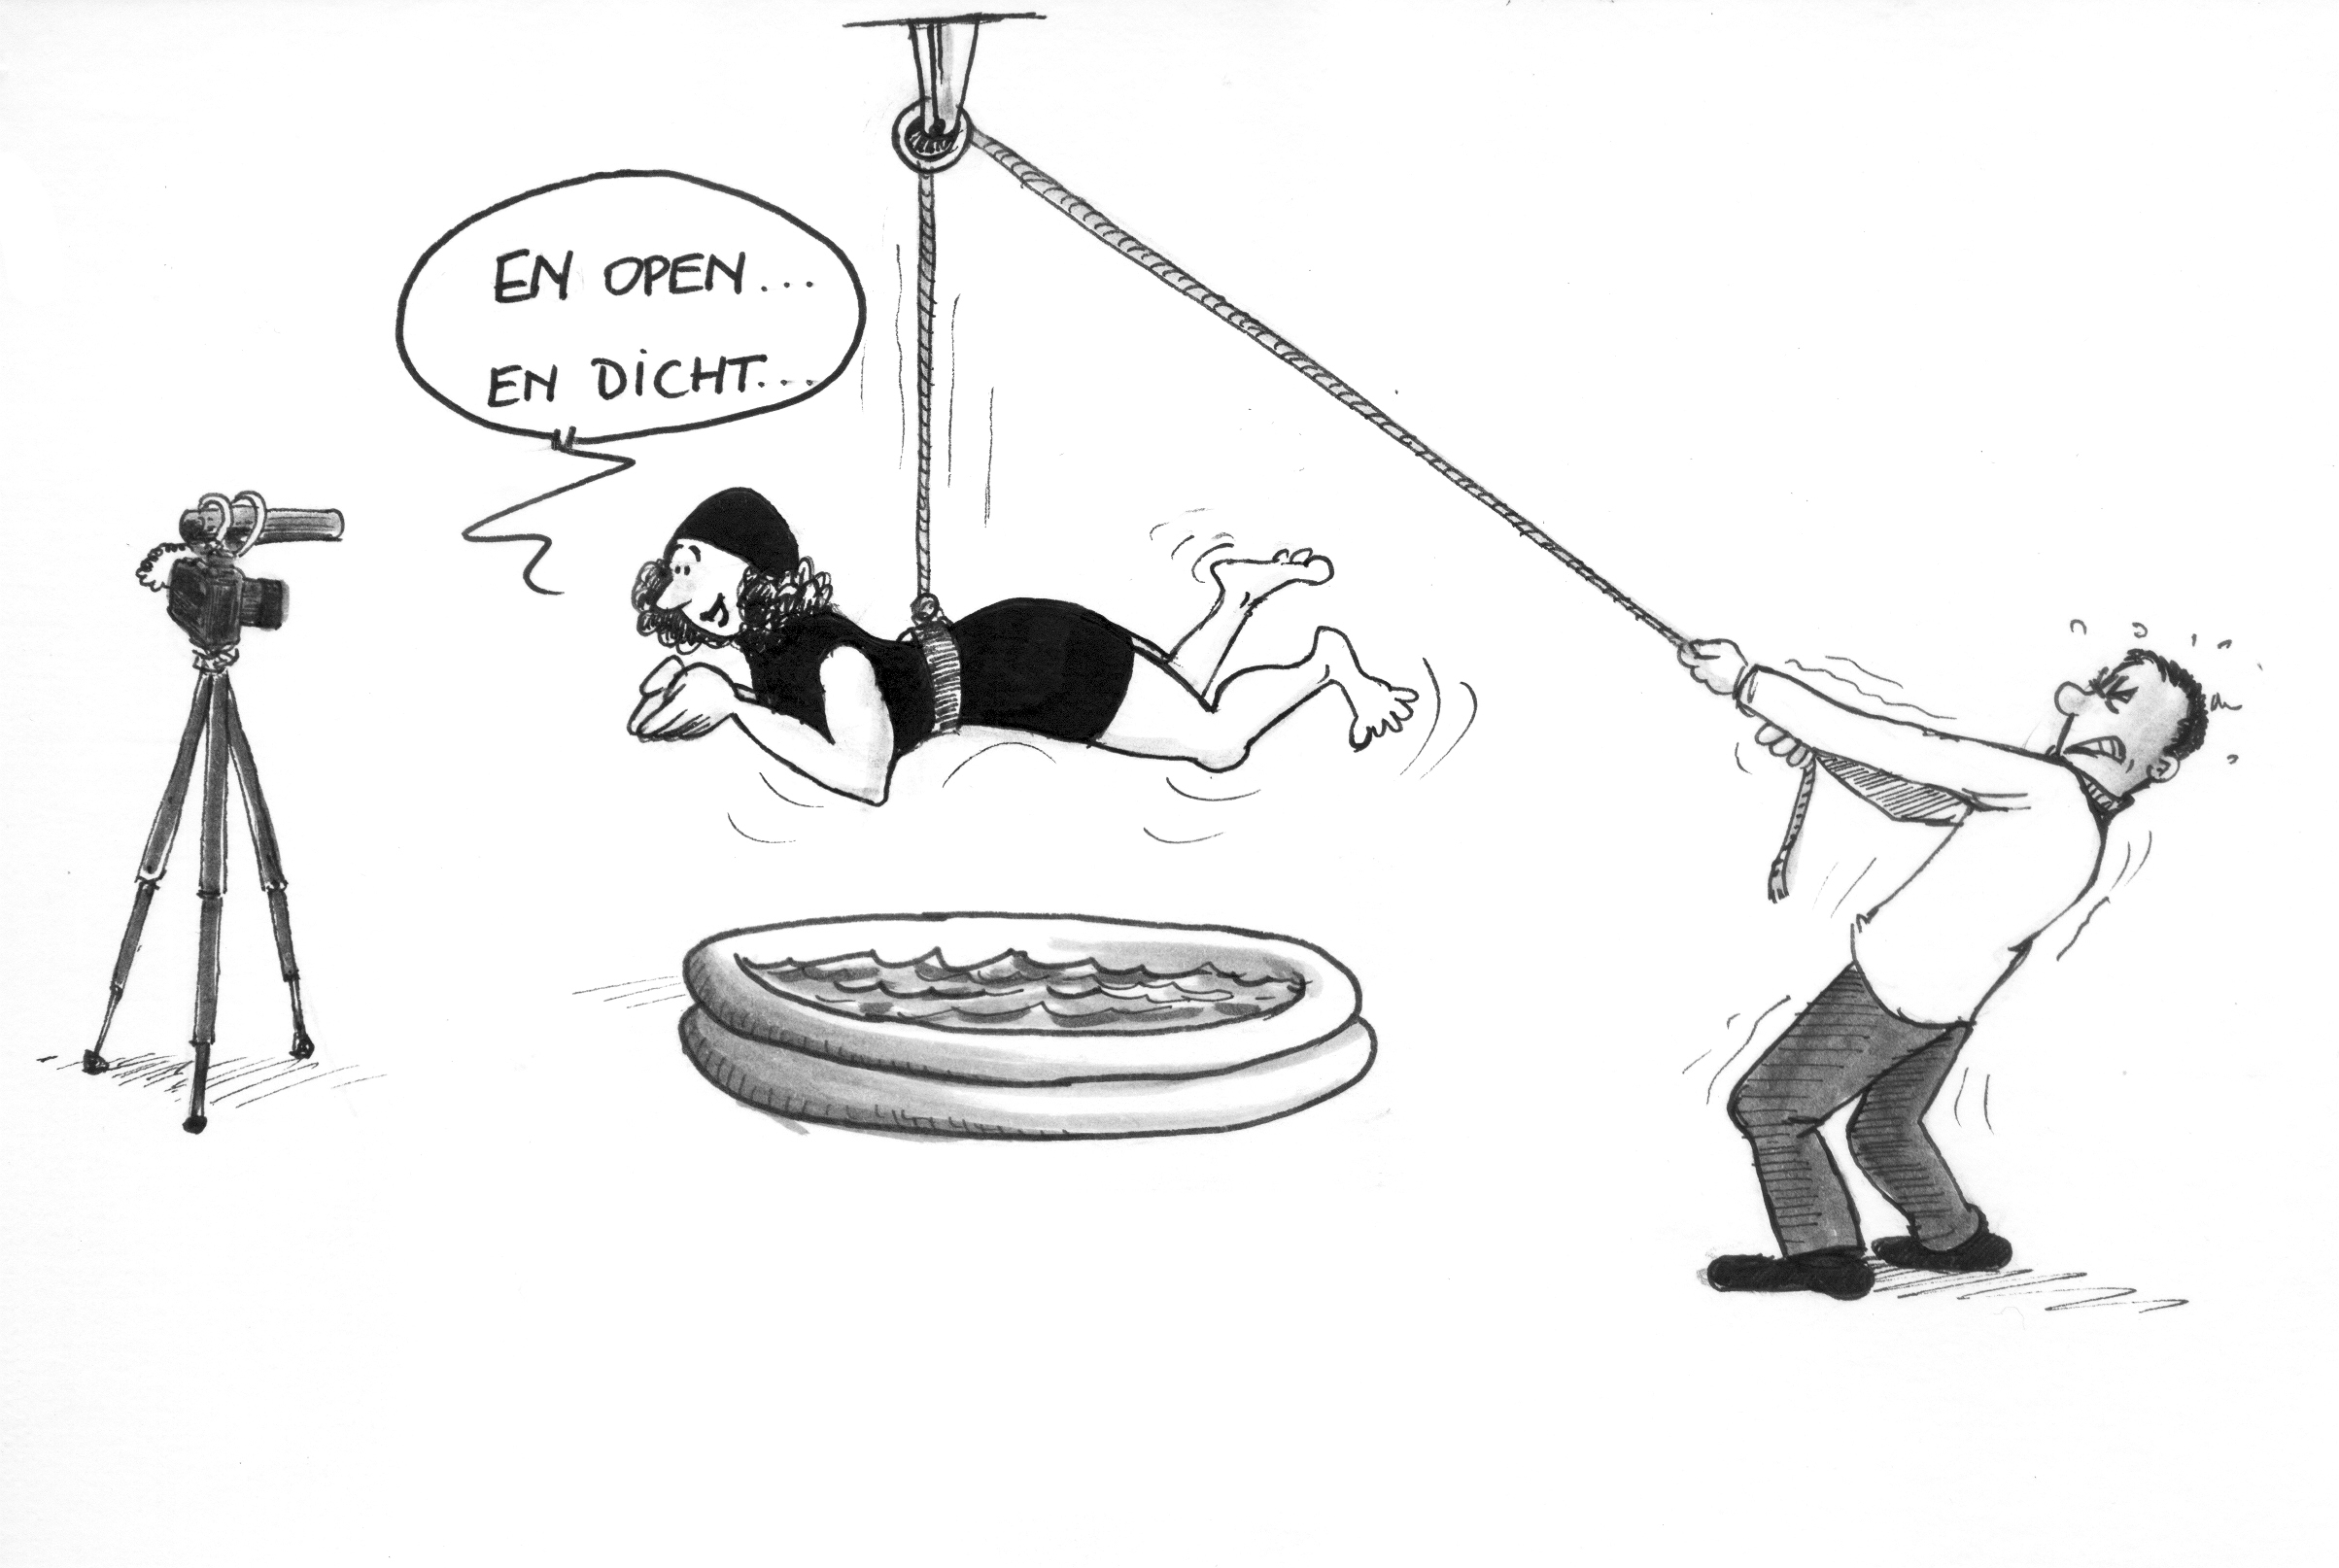
\includegraphics[width=14cm]{tekeningenKurt/uw november 2020 zwemmen.jpg}
\end{center}
\end{figure}

\begin{multicols}{2}
\subsection{Digitaal evalueren}

\emph{Maart 2020. Ik spreek met mijn collega af dat we intens willen samenwerken en vooral materiaal ontwikkelen dat we ook in niet-lockdown-tijden kunnen gebruiken. In het afstandsonderwijs missen we al snel het evalueren om het leerproces van onze leerlingen goed bij te sturen. Samen met een studente van de lerarenopleiding onderzoeken we digitale middelen die tijdelijk gratis hun maximale mogelijkheden aanbieden. We merken dat we in sommige tools zelfs feedback aan de leerlingen kunnen geven. Dit laat ons nadenken hoe we het leerlinggedrag bij het terugkrijgen van een toets kunnen veranderen. Vaak geven we een verbeterde taak of toets terug. De leerling bekijkt het cijfer, vergelijkt het met zijn buur, stopt het documentje al dan niet netjes in zijn boekentas om het dan niet meer te bekijken of erger nog, kwijt te spelen.}

`Feedback moet de kloof verkleinen tussen waar de leerling is en waar hij hoort te zijn.' Aan het woord is Hattie die het verband onderzocht tussen de onderwijsactiviteiten van de leraar en het leereffect bij leerlingen. Uit zijn onderzoek blijkt dat zowel feedback als formatieve evaluatie een wenselijk leereffect hebben. Goed evalueren, goede feedback geven opdat leerlingen leren uit hun evaluatie en iets met onze feedback doen, zijn zorgen die ons al ettelijke jaren bezig houden. We zoeken naar manieren om de focus minder op het cijfer te leggen, maar meer op het leren uit wat goed en fout is. 

Peter Johnston zegt: `Wanneer een cijfer onderdeel is van onze feedback, kijken studenten uit gewoonte niet verder dan het cijfer.' We herkennen dit en het is niet bemoedigend voor de leraar die veel feedback op de taak of toets schrijft. Een idee is om het cijfer pas achteraan op de toets te zetten. Van zodra leerlingen dat echter gewoon worden, is er geen verschil meer in hun gedrag. Een ander idee is om er een oefening van te maken en het cijfer in eerste instantie achterwege te laten. De leerling moet na het lezen van de feedback zelf zijn resultaat inschatten waarna hij het kan vergelijken met dat van de leraar.

De quote van Jan Chappuis `Effectieve feedback wordt gegeven tijdens het leren: op het moment dat je er nog iets mee kunt doen', ondersteunt de idee om regelmatig te evalueren. Feedback krijgen dient om  de opgedane kennis bij te schaven of te verfijnen. Tijdens het lesgeven in de klas geven we voortdurend feedback en krijgen we een globaal beeld van waar de groep staat. Hoe meer leerlingen in de klas hoe moeilijker het is om een goed beeld te krijgen van elk individu. Kleine toetsmomentjes tijdens het lesgeven maken zichtbaar hoe moeilijk het is om nieuwe kennis die je net onderwezen hebt, vast te houden. Nieuwe leerstof moet immers verwerkt worden en bij de ene leerling gaat dat sneller dan bij de andere. 

Toetsen en taken vormen van oudsher een onderdeel van onze onderwijspraktijk. De regelmaat waarmee we dit op individueel niveau doen, lijdt echter onder tijdsdruk. Goede toetsen opstellen en goede feedback geven waaruit de leerling kan leren om zichzelf te verbeteren, is tijdsintensief. Deze tijd is er doorgaans niet.

Het voorgaande maakt het belang van evalueren en feedback duidelijk. Tijdens het afstandsonderwijs moesten we plots overstappen naar een heel andere manier van onderwijzen. Om te `weten waar elke leerling is' konden we niet langer terugvallen op onze ervaring. Hoe moesten we dat doen bij het leren op afstand? Daarbij legde de overheid beperkingen op het evalueren van de leerstof tijdens het afstandsonderwijs. Leerlingen werden niet meer beoordeeld maar moesten des te meer zin hebben in leren en kennis verwerven. Dit vraagt gedragsverandering wat op korte termijn heel moeilijk en zelfs onmogelijk is. We zochten naar digitale middelen om ons hierbij te helpen. 

Sommige online middelen zijn bruikbaar om leerlingen te laten ervaren waar ze staan bij het verwerken van de leerstof en om hen een basisfeedback te geven die hen aan kan zetten tot het beter bereiken van de leerdoelen. Het is fantastisch dat je een toets kunt maken die zichzelf verbetert en waarbij je de leerlingen onmiddellijk feedback kunt geven. Dit spaart tijd uit voor de leraar, tijd die hij kan gebruiken om de feedback beter te richten op het leerproces van de groep en de individuele leerling. In wat volgt bespreken we enkele mogelijkheden om digitale huiswerken of toetsen op te stellen. We werkten met Kahoot!, Socrative en Google Formulieren. Andere collega's van de redactie ontdekten Quizizz en BookWidgets en misschien zijn er nog... veel betere... We realiseren ons dat deze tools continu evolueren. Hieronder lees je enkele voorbeelden over huiswerk en toetsen die we maakten tijdens de periode van maart tot juni 2020. Wellicht kunnen een aantal zaken ondertussen beter. We hopen de lezer te inspireren tot het onderzoeken van digitale middelen die kunnen werken in de eigen context.
\newpage

\tussentitel {Huiswerk op afstand opvolgen}

In de loep over telproblemen (UW 35/01) toonden we hoe je in Socrative een zelfverbeterende quiz kon maken. De leerlingen kregen telkens een korte feedback bij het juiste alternatief. We gebruikten de optie `Space Race' om een spelelement en wat competitie in de klas te brengen. 

Tijdens een online lesmoment kregen de leerlingen deze quiz als huiswerk op. Vanop mijn bureau kon ik via `Reports' en `Results' de voortgang van de leerlingen volgen. Ik zag hoever leerlingen stonden met het oplossen van de quiz en welke antwoorden ze kozen. Via rode en groen gekleurde cellen, kreeg ik een overzicht over foute en juiste antwoorden (figuur 1). Daarnaast kon ik een Excelbestand (figuur 2) exporteren dat de antwoorden toonde die elke leerling gekozen had.

\begin{center}
\includegraphics[width=\linewidth]{figurenAuteur/Socrative opvolgen leerlingen klein.png}
\captionof{figure}{Socrative: opvolgen van leerlingen}
\vspace{1 cm}
%\end{center}\
%\begin{center}
\includegraphics[width=\linewidth]{figurenAuteur/Excel Socrative antwoorden kleiner.PNG}
\captionof{figure}{Excel met antwoorden per leerling}
\vspace{-0.4 cm}
\end{center}\

Als herhalings- en evaluatietool gebruikte ik een kahootquiz (UW 35/01). Ook hier kon ik terugvallen op wat we voordien uitwerkten.

Door de optie `Assign a challenge' kunnen de leerlingen de quiz thuis maken op een moment dat hen past. Leraren kunnen een deadline vastleggen wanneer leerlingen ten laatste klaar moeten zijn en een timer instellen als ze willen dat leerlingen tegen tempo werken. Dat laatste vond ik minder geschikt als huiswerk omdat ik nauwkeurigheid boven tempo verkies en rekening wil houden met leerlingen die trager werken. Vragen per leerling in willekeurige volgorde laten verschijnen en een `nickname generator' aanzetten, zijn andere opties die je aan de context kunt aanpassen.

\begin{center}
\includegraphics[width=\linewidth]{figurenAuteur/Kahoot Assign a challenge.PNG}
\captionof{figure}{Kahoot en huiswerk}
\vspace{-0.2 cm}
\end{center}\

Eens de challenge is ingesteld, krijg je een URL om de quiz met de leerlingen te delen. Na de challenge vind ik via `Reports' per leerling een percentage van juiste antwoorden en het aantal niet beantwoorde vragen. 

Tijdens de lockdown maakten mijn collega en ik gebruik van de tijdelijk gratis Premiumversie waardoor we ook een overzicht kregen van vragen die moeilijk waren voor leerlingen. De analyse hiervan viel wat tegen. Het kwam er op neer dat Kahoot! de vragen die door de minste leerlingen juist werden opgelost, bestempelde als ´moeilijk'.

Toen we in september opnieuw live in de klas startten, borduurde ik op deze ervaringen verder. Nadat we in de klas rond het oplossen van kwadratische vergelijkingen gewerkt hadden, verwees ik voor het huiswerk naar opgaven op de website \url{https://wiskunde-interactief.be}. De leerlingen kregen als opdracht: 'Los de 15 oefeningen op tot je ze kunt. Je schrijft van elke soort oefening minstens 1 oefening met oplossing op huiswerkpapier.' Dat laatste voegde ik enkel toe om zicht te krijgen op hun inspanningen.  De volgende les begon ik met een kleine digitale quiz met gelijkaardige opgaven als in het huiswerk. 

Na maanden van afstandsleren merkte ik dat de drempel om digitaal aan het werk te gaan bij de leerlingen (en bij mezelf) veel lager lag dan voordien. Bovendien zorgde de digitale quiz ervoor dat ze onmiddellijk zicht kregen op de juistheid van hun antwoorden. Leerlingen die goed geoefend hadden, herkenden de opgaven van hun huiswerk. Zo ervaarden ze dat goed oefenen helpt om de leerstof te verwerken.

\newpage
\tussentitel{Digitaal toetsen}

Tijdens de eerste lockdown gebruikten we op onze school intensief Googleproducten. We leerden m.b.v. een instructiefilm van een collega, een toets opstellen met GoogleFormulieren. Op YouTube kun je via \url{www.youtube.com/watch?v=WMfa_kpr4GI} deze instructiefilm bekijken. Aanvankelijk waren we razend enthousiast over de eerder vermelde voordelen. Maar het vroeg doorzettingsvermogen. 

Mr. Google ondersteunt het gebruik van wiskundesymbolen niet. Spijtig genoeg kenden we op dat moment geen andere digitale tools die dat wel deden. We trotseerden echter de problemen. Alles wat een beetje wiskundig is, maakten we eerst in een Worddocument om er dan met een knipprogramma een knipsel (PNG-bestand) van te maken, allemaal vrij omslachtig. Het opstellen van zo'n toets is daardoor erg arbeidsintensief. 

Kenmerkend voor de mogelijkheden van digitale toetsen is hun gesloten karakter. Meestal stellen we op toetsen open vragen. We verwachten dat leerlingen hun antwoord op een logische en begrijpelijke wijze opschrijven. Bij het verbeteren stuiten we zo op typische denkfouten en op notatiefouten. Open vragen zoals een oefening oplossen, een redenering opbouwen, een opgave analyseren konden we niet opnemen in onze digitale toets. Bovendien zijn de mogelijkheden voor leerlingen om open vragen te beantwoorden weerom beperkt door de afwezigheid van wiskundesymbolen en de heel summiere lay-out mogelijkheden.

Dat laatste beperkte ons ook enorm in de wijze waarop we onze basisfeedback in de zelfverbeterende toets konden formuleren.

Maar toch waren wij en de leerlingen samen tevreden over deze manier van werken gezien de situatie. We kregen op die manier een indicatie over waar leerlingen in hun leerproces stonden. Aan de hand van enkele voorbeelden uit de toetsen die we opstelden tijdens de eerste lockdown, tonen we hier mogelijke vraagvormen en hoe we beoordeelden en feedback gaven. Bij het opstellen hielden we steeds in het achterhoofd dat we vooral wiskundig denken willen evalueren. Een methode vinden we belangrijker dan een resultaat en dit willen we ook met onze feedback en het behaalde cijfer ondersteunen.

\end{multicols}

\beginwerktekst{Vraagvormen, punten en feedback bij een toets in GoogleFormulieren}
\begin{werktekstoef}
\item{Meerkeuzevraag}

\begin{center}
\includegraphics[width=10cm]{figurenAuteur/Foto's invoegen.png}
\captionof{figure}{Een samengesteld combinatorisch probleem}
\end{center}\

De opgave is een meerkeuzevraag over de attracties in Bobbejaanland. De tabel met attracties is een voorbeeld van een foto die je bij de vraag moet invoegen. Het is een vraag over telproblemen in de derde graad. We belichten bij deze vraag de alternatieven en het toekennen van punten.

De getallen die in de alternatieven voorkomen zijn weloverwogen gekozen. De leerling moet de juiste keuze maken voor de indices, de juiste keuze tussen een aantal variaties (V) of combinaties (C) en de juiste keuze tussen optellen en vermenigvuldigen. Zo kom je, naast het correcte antwoord, tot relevante afleiders.
\begin{opsomming}
\item$965=V_7^4+V_6^3+V_5^1$
\item$3005=C_7^4 \cdot C_6^3 \cdot C_5^1$
\item$504000=V_7^4 \cdot V_6^3 \cdot V_5^1$
\item$2593080=7^4 \cdot 6^3 \cdot 5$
\end{opsomming}
Door de meerkeuzevragen op meer dan 1 punt te zetten, geef je jezelf ruimte voor enige nuance bij het verbeteren waarbij je voor de ene afleider nog een punt geeft en voor de andere niet. In de figuur zie je rechtsboven dat er 2 punten te behalen zijn. Leerlingen die het derde alternatief markeren krijgen 2 punten. Het eerste alternatief verdient 1 punt omdat de leerling het deelprobleem juist oplost maar de foute keuze maakt tussen optellen of vermenigvuldigen en dus de productregel niet goed begrijpt.

Je kunt in twee stappen werken. Leerlingen krijgen van zodra ze de toets afgeven de automatische beoordeling met feedback. Vervolgens stuur je de verbetering bij en krijgen de leerlingen een definitieve score. Na de eerste toets wisten de leerlingen dat hun resultaat na een tweede verbetering hetzelfde of hoger zou liggen. 

Je kunt er ook voor kiezen om het resultaat met feedback niet onmiddellijk te geven als je wilt vermijden dat juiste antwoorden gedeeld worden vooraleer alle leerlingen klaar zijn. Dit is uiteraard in tegenspraak met de kracht van onmiddellijke feedback. Feedback die de leerling krijgt wanneer hij zijn antwoorden en redeneringen nog vlot terug kan oproepen, werkt doorgaans beter. 

\item{Selectievakjes}

\begin{center}
\includegraphics[width=12cm]{figurenAuteur/Selectievakjes met antwoord.PNG}
\captionof{figure}{Selectievakjes}
\end{center}
Een vraag met vierkante selectievakjes lijkt op een meerkeuzevraag met dit verschil dat meerdere alternatieven juist kunnen zijn. Het voorbeeld hierboven toont een vraag over het onderwerp van de normale verdeling. We belichten met deze vraag hoe je het antwoordmodel maakt, hoe je feedback kunt geven en hoe je punten kunt geven. 

Rechtsboven zie je dat de leraar deze vraag op 3 punten zet (via de pijltjes kun je het totaal te behalen punten aanpassen). Hij vinkt de juiste alternatieven aan. Onderaan kan hij feedback noteren die de leerling te zien krijgt als hij een afwijkend antwoord geeft t.o.v. de twee aangevinkte vakjes. Ook hier kun je merken hoe beperkt van wiskundige symboliek en het opstellen van feedback is.

De automatische verbetering is overdreven streng. Als de leerling de 2 juiste alternatieven aanvinkt, krijgt hij 3 punten. Maar als hij één van beide juiste alternatieven niet aanklikt, kent de automatische verbetering 0 punten toe. De digitale tool legt geen nuances. Je kunt dit echter aanpassen en met een antwoordmodel werken. Met het antwoordmodel kan deze leraar 2 punten geven voor alternatief 4 en 5. Dat is verantwoord omdat de leerling één alternatief juist aanvinkt en wel weet dat invNorm de juiste instructie is, maar een fout maakt tegen het percentage. Hij kan tenslotte 1 punt geven voor 1 juist alternatief. Bij dit soort vragen moet je zeker de automatische verbetering nakijken en aanpassen.

\item{Meerkeuzeraster}

Een meerkeuzeraster vraagt om verbanden te leggen. Per rij en kolom kan de leerling meerdere keuzes aanvinken. Het voorbeeld hieronder toont het antwoordmodel bij een vraag uit het onderwerp kansrekenen. De beperking bij deze ingebouwde vraagvorm is dat er geen optie voorzien is om feedback te geven.
\begin{center}
\includegraphics[width=12cm]{figurenAuteur/Meereuzeraster 3.PNG}
\captionof{figure}{Meerkeuzeraster}
\end{center}\

\item{Kort antwoord of alinea}

Een laatste soort vragen die ik gebruikte zijn de `kort antwoord- of alineavragen'. Ik gebruikte ze niet voor open wiskundige vragen omdat ook de leerlingen geen wiskundige symbolen kunnen gebruiken in hun antwoorden. Met deze vragen ging ik na hoelang leerlingen gestudeerd hadden, of ze de toets met hun boek en notities hadden gemaakt of niet,  hoelang ze aan de toets gewerkt hadden, of ze suggesties hadden voor het afstandsonderwijs en andere gevoelsmatige vragen.
\begin{center}
\includegraphics[width=\linewidth]{figurenAuteur/open vraag.PNG}
\captionof{figure}{Open vraag}
\end{center}\

\item {Verplichte vraag}

Tot slot heb je de mogelijkheid om vragen te verplichten of vrij te laten. Die kan je gebruiken wanneer leerlingen verschillende leerstof doornamen of met een verschillend tempo toetsen oplossen. Het voorbeeld hieronder toont zo'n vraag over het sommatieteken, leerstof die niet voor elke leerling nodig en zinnig was. Ook in deze vraag merk je elementen die we al hiervoor bespraken: punten en wiskundige symbolen die je elk apart als foto moet invoegen.
\begin{center}
\includegraphics[width=12cm]{figurenAuteur/Vragen niet verplicht.PNG}
\captionof{figure}{Wiskundige symbolen invoeren}
\end{center}\
\end{werktekstoef}
\eindewerktekst

\begin{multicols} {2}
Zoals je kon lezen liepen we tijdens het opstellen van digitale toetsen tegen een aantal problemen aan. Het maakte helder wat we wilden en zorgde ervoor dat we creatief moesten nadenken over toetsvragen die toetsten wat wij wilden weten. Dat gaf ons nieuwe inzichten. De kennis die we daarbij opdeden kunnen we inzetten bij het opstellen van gewone toetsen. Sommige gesloten vraagvormen die onze digitale tool toeliet, waren nieuw voor ons en leerden ons verder denken over andere manieren van vragen stellen. Deze nieuwe vraagvormen kunnen we natuurlijk ook gebruiken in offline onderwijs.

We zijn op een grondigere manier gaan kijken naar gesloten vragen. Het is een uitdaging om gesloten vragen of meerkeuze vragen zo te maken, dat leerlingen die een goede redenering opbouwen, het juiste alternatief (antwoord) kiezen en leerlingen die dat nog niet kunnen een fout alternatief (afleider) kiezen. Weloverwogen alternatieven zoeken, is de boodschap. Je moet ervoor zorgen dat een antwoord met een typische denkfout voorkomt in de afleiders. Op die manier komt het aan het licht als een leerling een denkfout maakt. Het opstellen van goede alternatieven laat je nadenken over dit soort denkfouten. Dit helpt om je instructie beter in te vullen.

Een tweede uitdaging was het op voorhand kritisch nadenken over wat we willen toetsen en dit naast de gesloten vragen leggen. Een gesloten vraag kan onbedoeld bepaalde mechanismen in het werk zetten. 

Zo kan een leerling in de berekening een fout maken en zijn antwoord niet terugvinden tussen de alternatieven. Als hij opnieuw gaat rekenen en blijft rekenen omdat hij zijn fout niet vindt, zal dit tijdverlies zijn. 

Een ander probleem is dat meerkeuzevragen aanleiding kunnen geven tot het zogenaamde `terugwerken vanuit de alternatieven'. Alhoewel dat op zich een zinvolle heuristiek is om te beheersen, toetsen we dan niet of de leerling het leerdoel bereikt. Een typisch voorbeeld is een algebra-opgave waarbij de leerling een lineaire vergelijking met één onbekende moet oplossen. Wanneer je in de meerkeuzevorm verschillende oplossingen geeft (juiste en foute), hoeft de leerling enkel deze getallen in de vergelijking te substitueren om het correcte alternatief te vinden. We meten dus iets anders dan bij een open vraag. Het is goed om je ervan bewust te zijn dat je mogelijk niet weet hoe de leerling het antwoord vond: met een schatting, een gok of een berekening.

Een digitale toets automatiseert het verbeteren en het geven van feedback. Hoe vaardiger de leerlingen (en wijzelf) met online tools zijn, hoe minder tijd er verloren gaat naar praktische organisatie. Deze evaluatievorm is dus uitermate geschikt om regelmatig kort tussentijds te evalueren. Door een intro- of exit-ticketje of een kort evaluatiemoment in een les wordt het regelmatig nakijken `waar elke leerling staat' haalbaar. 

Daarnaast kun je de wiskundige onbekwaamheid van Mr.Google opvangen met enkele digitale tools die we jammer genoeg nog niet kenden in de eerste lockdowm. In Quizizz en BookWidgets kun je vergelijkbare soorten vragen maken. Het grote voordeel is echter dat je in deze tools wel wiskundige symbolen kunt typen. Quizizz is gratis en heeft een `wiskundige vergelijkingseditor'.

\begin{center}
\includegraphics[width=\linewidth]{figurenAuteur/quizizz editor.png}
\captionof{figure}{Wiskundige schrijven in Quizizz}
\end{center}

De basissymbolen zijn uitgebreid met het Griekse alfabet en een set gevorderde symbolen zoals doorsnede, verschillende pijlen en andere wiskundige symbolen. Alexandra Verbuyst maakte een instructiefilmpje dat je wegwijst in de wondere wereld van Quizizz. Je kunt het bekijken op YouTube via de volgende link: \url{www.youtube.com/watch?v=3HrTWBMFVUA&t=952s&ab_channel=AlexandraVerbuyst}.

\begin{center}
\includegraphics[width=\linewidth]{figurenAuteur/quizizz vergelijkingseditor.PNG}
\captionof{figure}{Vergelijkingseditor in Quizizz}
\end{center}

BookWidgets is een betalend programma. Je kunt het eenmalig gratis voor een maand uitproberen. Het zal je niet verwonderen dat dit nog heel wat meer mogelijkheden heeft. Zo kun je om toetsen op te stellen, kiezen uit 25 soorten vragen. Je kunt wiskundige symbolen typen, al vergt dat een beperkte kennis van LaTeX. Leerlingen kunnen een antwoord op het whiteboard schrijven. 

\begin{center}
\includegraphics[width=\linewidth]{figurenAuteur/Bookwidgets white board vraag.PNG}
\captionof{figure}{Leerlingen schrijven op het bord}
\end{center}

Voor scholen die met Smartschool als leerplatform werken, is het vlot toegankelijk via de module `Oefeningen' en worden punten automatisch in Score toegevoegd. Over BookWidgets kun je heel wat handleidingen raadplegen. Op de website van Uitwiskeling staat een handleiding, geschreven door een collega, met de belangrijkste LaTeX commando's die je nodig hebt om vlot met BookWidgets te werken.

\begin{center}
\includegraphics[width=\linewidth]{figurenAuteur/Bookwidgets en smartschool.PNG}
\captionof{figure}{BookWidgets en Smartschool}
\end{center}
\end{multicols} 

In de onderstaande tabel vatten we enkele mogelijkheden van de onlinetools samen.
\vspace{0.5 cm}

\begin{tabular}{|l|c|c|c|c|c|}
\hline
\textbf{Wat?}  & \textbf{Kahoot!}  & \textbf{Socrative}  & \textbf{Google Forms}  & \textbf{Quizizz}  & \textbf{Bookwidgets} \\
\hline
Gratis  & x  & x  & x  & x  & o  \\
\hline
Wiskunde symbolen  & o  & o  & o  & x  & x \\
\hline
Meerkeuzevragen  & x  & x  & x  & x  & x  \\
\hline
Selectievakjes  & o  & x  & x  & x  & x  \\
\hline
Meerkeuzeraster  & o  & o  & x  & o  & x  \\
\hline
Korte antwoorden  & o  & x  & x  & x  & x  \\
\hline
Meer dan 5 vraagvormen  & o  & o  & o  & o  & x  \\
\hline
Blanco vak invullen  & o  & o  & x  & o  & x  \\
\hline
Lln. kunnen wisk. noteren  & o  & o  & o  & o  & x  \\
\hline
Lln. kunnen knn foto uploaden  & o  & o  & ?  & ?  & o  \\
\hline
Zichzelf verbeterend  & x  & x  & x  & x  & x  \\
\hline
Leraar kan voortgang volgen  & x  & x  & o  & ?  & ?  \\
\hline
Tijdslimiet per vraag  & 120 s  & o  & 15 min.  & ?  & x  \\
\hline
Gedetailleerd verslag resultaten  & o  & x  & x  & ?  & ?  \\
\hline
\end{tabular}
\vspace{1 cm}

\begin {multicols}{2}
\subsection{Onlinegroepswerk}
\emph{Ik ben geen fan van doceren. Ook al kan een kort gestructureerd doceermoment erg verhelderend zijn en de hersenen van mijn leerlingen aan het werk zetten, het is niet mijn favoriet. Ik vond het niet eenvoudig om via een scherm mijn leerlingen te activeren. Daarnaast bleef ik zoeken naar manieren om mijn verbeterwerk binnen de perken te houden. De zoektocht naar oplossingen voor deze twee bekommernissen leidde tot een onlinegroepswerk waarin leerlingen samenwerkten in één Google Document. Ik heb het tweemaal uitgeprobeerd maar ben nog niet helemaal tevreden over mijn ontwerp en het resultaat. Ik neem je mee in mijn zoektocht.}

In sommige software zoals Zoom en Blackboard Collaborate Ultra kan je via `breakout rooms' of `parallelgroepen' je onlineklas vlot in groepen verdelen. Jammer genoeg, werd dit in onze school niet gebruikt. 

We werkten al langer met Google Suite waardoor we meer mogelijkheden hadden met Google producten zoals Classroom en Meet wat in de gratis versie `Hangouts' heet. De onlinelessen gaven we via Google Meet met een vaste `Meet-ruimte' voor elke klas en het advies om de lessen op te nemen. In Google Meet kon ik de leerlingen echter geen aparte werkruimte per groepje geven. Wat googelen leverde een oplossing. Elke groep kreeg een eigen link en code voor hun persoonlijke ´Meet-ruimte'. Het werd een les met een complementair groepswerk. Elke groep kreeg eigen oefeningen toegewezen. Ik plande het zo dat elke oefening niet door alle, maar wel door verschillende groepen gemaakt werd. Hieronder lees je de instructie voor het groepswerk.
\end{multicols}
\newpage

\beginwerktekst{Onlinegroepswerk}

De instructie voor de volgende 15 minuten van de les. 
\begin{nummering}
\item Je werkt in groepen in een eigen Google Meet-ruimte. Alle groepen werken in hetzelfde Google Document.
\item Open het gedeelde Google Document. 
\item Duid een verslaggever in je groep aan die de oefening aan de rest van de klas kan uitleggen als we terug verzamelen in de hoofdruimte.
\item We maken in deze les de volgende acht oefeningen: 17, 18, 44, 46, 47, 51, 55, 57. Elke groep krijgt een eigen set van oefeningen. Elke oefening wordt door minstens twee groepen opgelost.

\indent Groep 1: Camryn, Quinten, Sander, Nette, Jesper
OEFENING 17, 47, 57

\indent Groep 2: Jens, Robbe, Helen, Lisa, Charlotte		
OEFENING 18, 47, 57

\indent Groep x: xxx

\item Je maakt zeker de eerste oefening die ik voor jullie groep selecteerde. Ben je hiermee klaar dan maak je de andere oefeningen.
\item De oplossingen van de oefeningen verzamelen we in het gedeelde document. Elke oefening heeft een eigen bladzijde. Voeg een foto van je oplossing toe of schrijf deze op de juiste bladzijde. 
\item Hieronder vind je je eigen groepslink. Ik heb alle ‘Meets’ open staan en kan langskomen. Klik de link aan vanuit je school-e-mailadres.

\indent Groep 1: https://meet.google.com/wzz-qhzt-brk code g1

\indent Groep 2: https://meet.google.com/qrt-avtq-tco code g2

\indent Groep x: xxx

\end{nummering}
\eindewerktekst
\begin{multicols} {2}

Ik was aangenaam verrast hoe goed de leerlingen in hun ruimte samenwerkten. Ik passeerde er en hoorde hen in hun taaltje converseren en overleggen over de oefeningen. Sommige leerlingen die ik anders veel minder hoorde, waren nu erg aanwezig en deden hun zeg bij het oplossen van de oefeningen. 

Niet alles liep perfect, wat te verwachten was in mijn klas en met een werkvorm die ik nog nooit gebruikte. Sommige groepen deelden in het gemeenschappelijke document een oplossing zodra een oefening klaar was. Andere groepen moest ik hiertoe aansporen. Sommige groepen voegden hun oplossing in op een foute plaats in het document. 

\end{multicols}


\begin{figure}[H]
\begin{center}
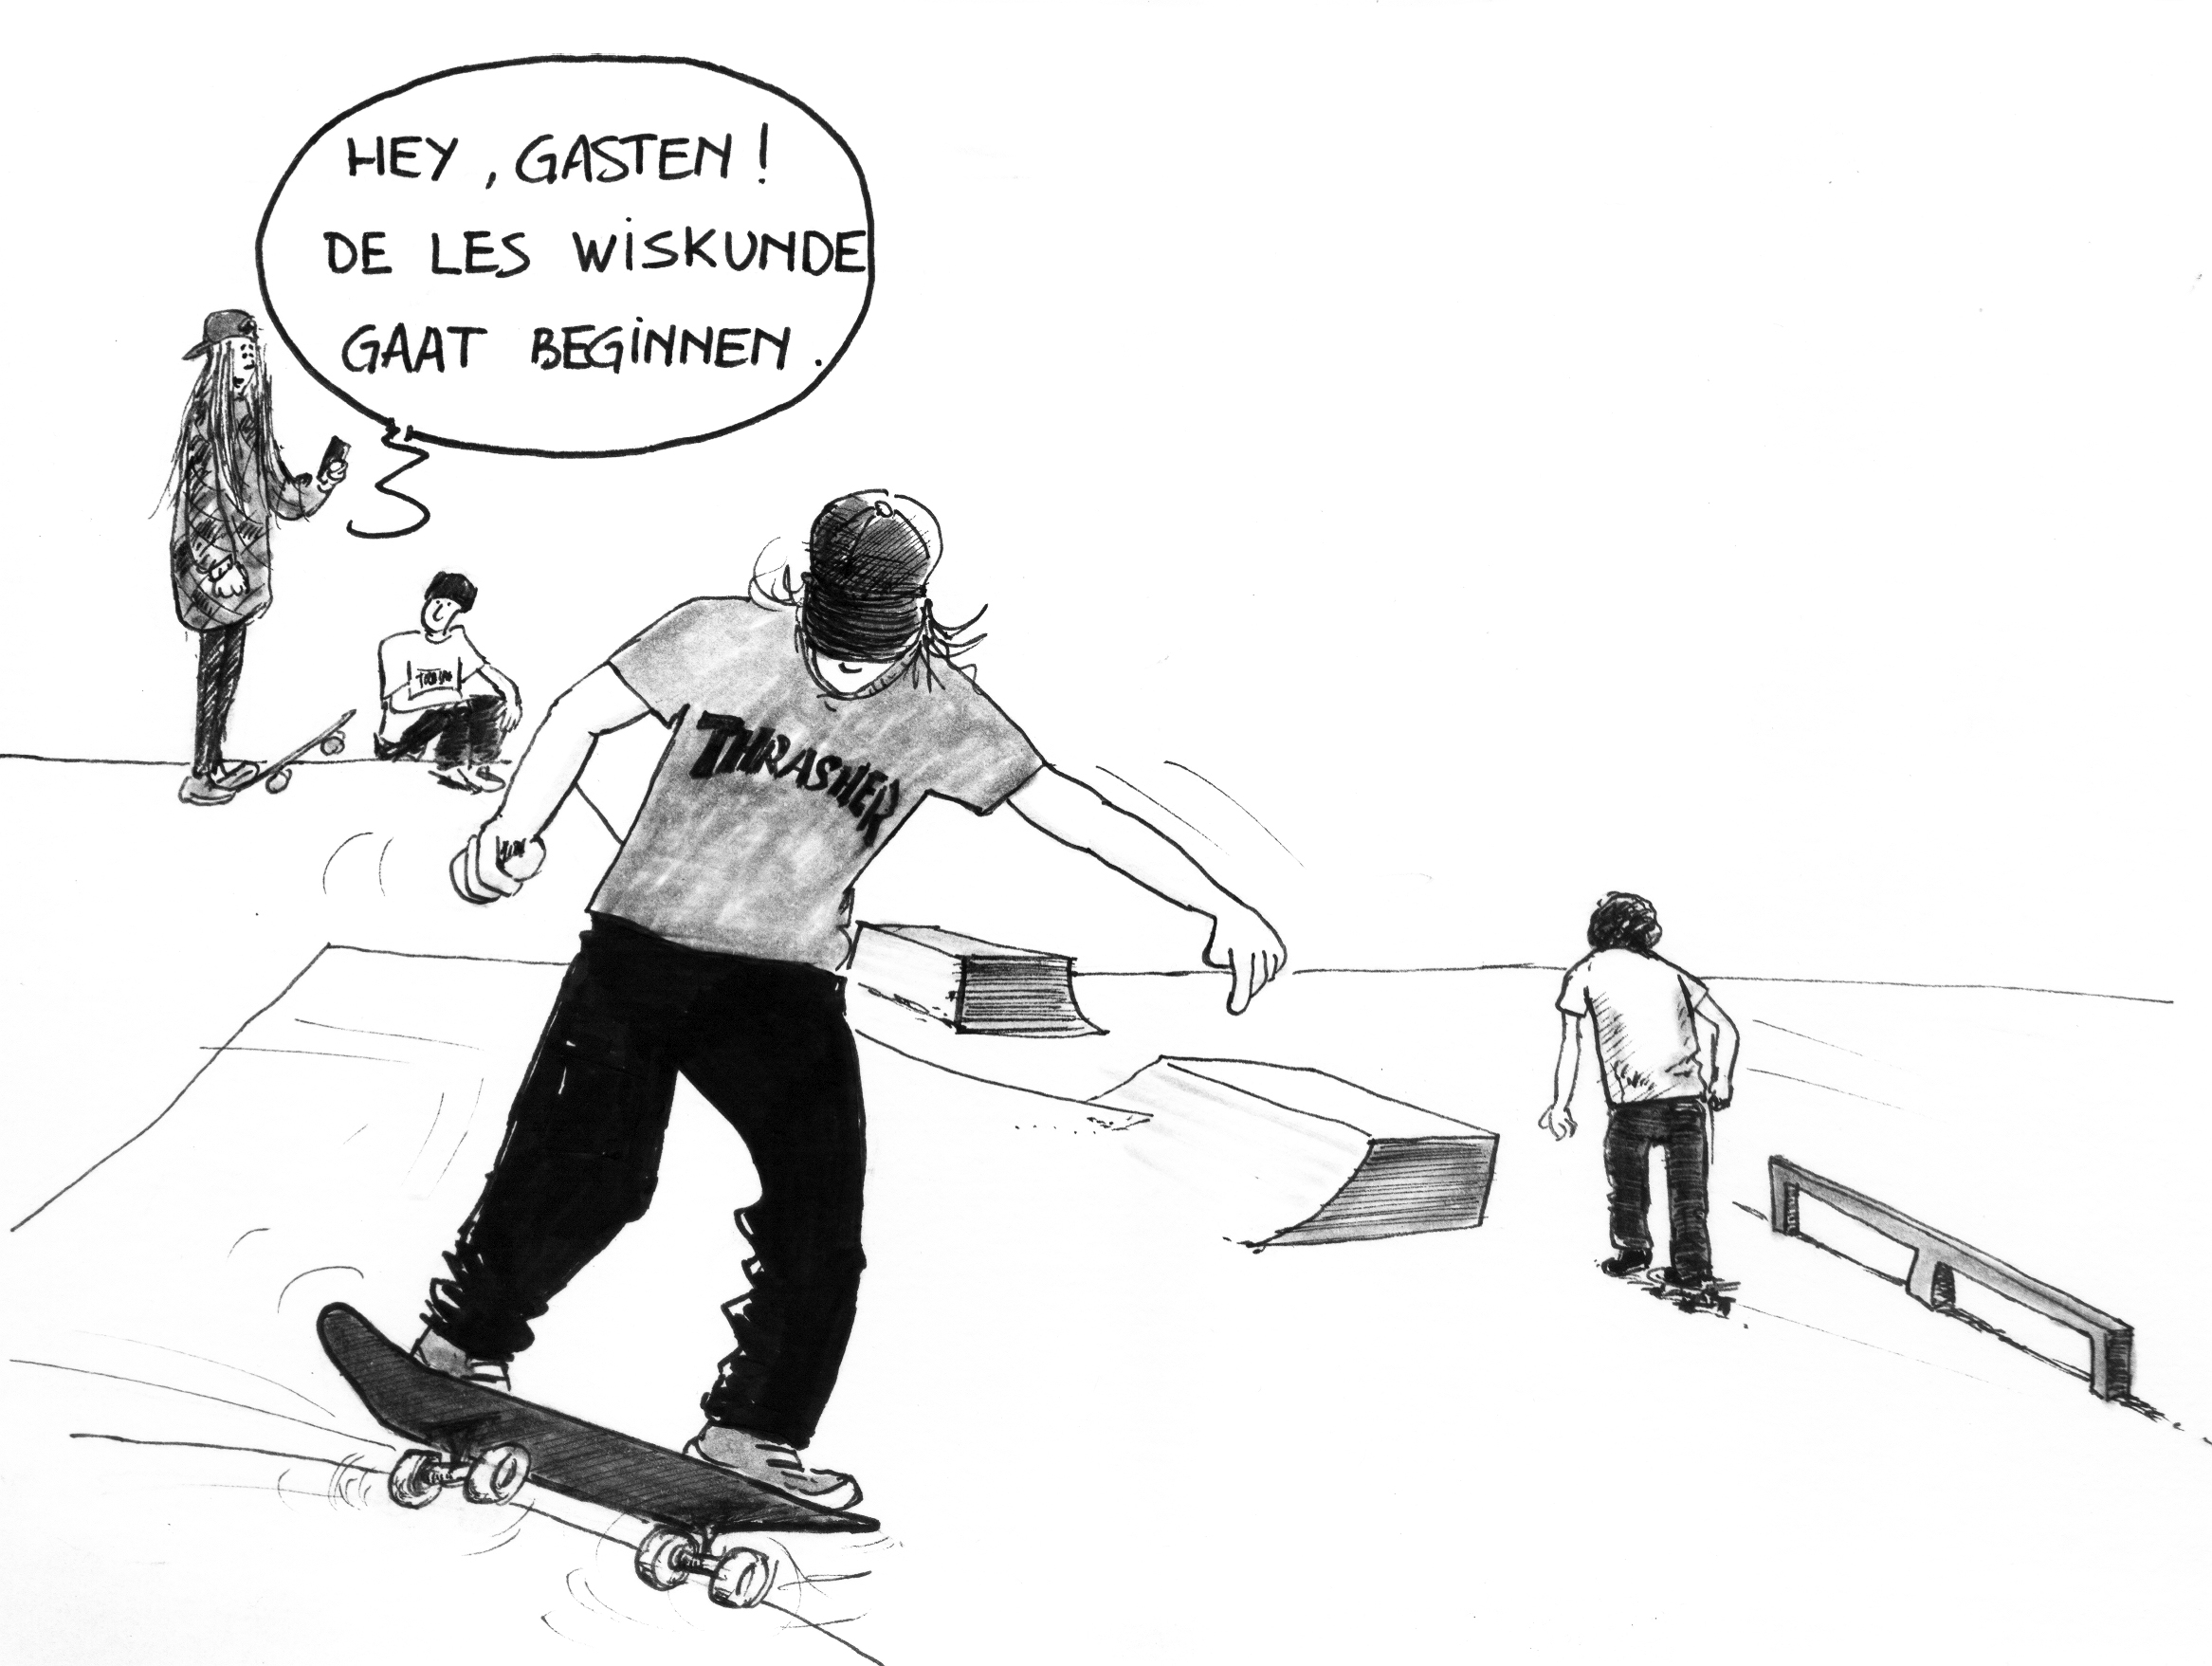
\includegraphics[width=10cm]{tekeningenKurt/uw november 2020 skaten.jpg}
\end{center}
\end{figure}

\begin{multicols}{2}

Het lastigste was dat ik alle Meet-sessies tegelijk in mijn koptelefoon hoorde, waardoor interactie met één groepje bijna onmogelijk was. Maar ondertussen kun je ook in Google Meet vlotjes je klas in groepen delen. De ene digitale tool haalt duidelijk de andere tegen een sneltempo in. 

De figuur hieronder toont een typisch beeld als leerlingen hun video niet graag aanzetten. In sommige groepen `floepten' de video's aan tijdens het groepswerk, in andere niet. Ik liet mijn leerlingen hier vrij in, al vond ik het wel leuk om ze effectief bezig te zien. 

\begin{center}
\includegraphics[width=\linewidth]{figurenAuteur/Google meet groepswerk.png}
\captionof{figure}{Meet-sessie}
\end{center}

Tevreden blik ik op dit eerste probeersel terug. De leerlingen waren nog nooit zo zichtbaar actief geweest tijdens een onlineles. Zelf had ik minder verbeterwerk én het was eenvoudiger. Ik moest immers slechts één document openen en corrigeren. In dit document becommentarieerde ik telkens maximum twee oplossingen van eenzelfde oefening, in totaal 16 uitgewerkte oefeningen. Ik gaf mijn feedback en gebruikte hierbij fotootjes van de oplossingen uit het handboek. De figuren hiernaast tonen een opgeloste oefening van een groepje en het antwoordmodel van het boek. 

Ik gaf een uitgebreide feedback in het gedeelde document. In de oplossing van de leerlingen merk je dat ze twee methodes uitproberen. Een methode waarbij ze nieuwe leerstof gebruiken (telproblemen) en vastlopen doordat ze een fout maken. Ze schakelen dan over naar een methode die ze al leerden in het vierde jaar (en maken een fout). Ik wijs hen op wat goed is, verwijs naar de nieuwe methode en waar ook het antwoordmodel van het boek gebruik van maakt. Hier stuit ik op de schraalheid van verbetersleutels die slechts één methode weergeven zonder enige nuance. 


\begin{center}
\includegraphics[width=\linewidth]{figurenAuteur/Oplossing in google doc.png}
\captionof{figure}{Oplossing in gedeelde document}
\end{center}
\begin{center}
\includegraphics[width=\linewidth]{figurenAuteur/Google Doc Opgave met antwoordmodel.png} 
\captionof{figure}{Antwoordmodel van het boek}
\end{center}

\tussentitel{Leerlingen leren van feedback}
\emph{Mijn zoektocht liep verder en richtte zich op het geven van feedback. Twee vragen die me ook in `niet-lockdowntijden' bezig houden, staken terug de kop op: `Hoe zorg ik er voor dat mijn leerlingen iets doen met mijn feedback? Hoe leer ik leerlingen fouten verbeteren?'}

In maart spraken we op schoolniveau af dat leerlingen hun werk zouden afgeven in Google Classroom. Je kunt dan vlot van het document van de ene leerling naar dat van de andere springen. De chatfunctie laat toe om te communiceren met leerlingen. 

Tijdens de lockdown had ik heel wat meer gerichte taak-gesprekjes met leerlingen dan in een klassikale setting. Wat ik heel handig vind in `Classroom' is dat je de commentaar die je schrijft in een reactieoverzicht kunt opslaan. Als je nadien een woord typt dat je al eerder gebruikte in een commentaar, kun je deze commentaar eenvoudig terug oproepen, hergebruiken of herwerken. Figuur 16 op de volgende bladzijde toont zo'n reactieoverzicht.
\end{multicols}

\begin{center}
\includegraphics[width=\linewidth]{figurenAuteur/Feedback en reactieoverzicht.png}
\captionof{figure}{Feedback hergebruiken}
\vspace{-0.2 cm}
\end{center}


\begin{multicols} {2}
De volgende opdracht was een bescheiden poging om leerlingen aan te zetten tot het kritisch kijken naar oplossingen. Ik liet ze een tweede maal in één document werken en zette hen aan oplossingen van een andere groep te bekijken en te verbeteren. Ondertussen naderde de vakantie en ging 6 EMT zijn laatste twee weken afstandsonderwijs in. Toch gaf ik nog niet op, zocht ik verder en gaf hen de volgende instructie.

\end{multicols}
\beginwerktekst{Onlinegroepswerk - Geef elkaar feedback}

Werk samen aan de oefeningen die in de opdrachtenkaart van hoofdstuk 4 staan. Naast de Meet-link die in Google Classroom blijft openstaan, kun je andere digitale tools uitproberen waarmee je vlot met elkaar kan communiceren, je scherm delen enz… (discord.com, zoom.us, www.praatbox.be, messenger, WhatsApp...).

Open het gedeelde document waarin je met alle groepen samenwerkt. Je vindt er de groepsindeling. De groepsleider is vetgedrukt. Hij/zij is ervoor verantwoordelijk dat jullie groep in orde is. Je mag een andere groepsleider kiezen. Geef zijn naam dan een groene kleur. Je mag ook de groepen herindelen, maar het aantal leerlingen per groep mag niet wijzigen. Veranderingen tussen groepen doe je in een rode kleur.

Je vindt in het document de oefeningen die je met je groep moet maken. Elke oefening wordt gemaakt door twee groepen. Zet de oplossing van je groep in het document EN geef feedback bij de oplossing van de andere groep die dezelfde oefening maakte. Duid fouten aan en interessante werkwijzen. Je kunt dit doen door in de kantlijn commentaar te geven. 

Maak heel duidelijke foto’s, zodat je het elkaar niet lastig maakt om de foto te kunnen lezen.

In het gedeelde document vind je vooraan een `vragenbladzijde'. Noteer hier vragen die je hebt. Iedereen die een antwoord weet, of denkt te weten, kan antwoorden op de vragen van medeleerlingen en iedereen kan mee volgen. 

Als het me lukt, zal ik het document af en toe bekijken en ook commentaar geven. Ik beloof echter niets en reken op jullie verantwoordelijkheidszin.

\eindewerktekst

\begin{multicols} {2}
Het groepswerk liep terwijl ik in ziekteverlof was. Ik had mijn afwezigheid zorgvuldig tijdens de examens gepland... maar corona besliste dat we tot half juni zouden lesgeven.

Opnieuw verrasten mijn leerlingen me, al was het geheel toch te pover voor wat ik voor ogen had. Eerlijk gezegd had ik verwacht dat er vanaf mijn afwezigheid niet veel meer zou gebeuren want laat ons eerlijk zijn `een leerling zonder leraar is als een dak zonder dakpannen'. Mijn leerlingen bleven echter bezig en vulden het document met hun oefeningen. Meer dan dat gebeurde er echter niet. Een groep las de instructie niet goed en leverde een oefening in van het vorige hoofdstuk. Verder hebben ze niet veel van elkaar verbeterd, lazen ze de feedback die ik tussendoor gaf niet en bleef de vragenbladzijde maagdelijk leeg.

De ervaringen tijdens deze zoektocht leerden me toch een aantal elementen die ik zeker wil vasthouden ´in mijn gewone onderwijspraktijk'. 

Het werken in één gedeeld document is voor mezelf erg efficiënt bij het verbeteren. Daarnaast is het een enorme meerwaarde dat mijn feedback in één document staat dat voor alle leerlingen toegankelijk is. 

Het online indienen van documenten via Google Classroom is me enorm bevallen en wil ik behouden. Ik kon op de duur zonder al te veel extra inspanningen mijn leerlingen veel meer gerichte feedback geven. Het paste wel bij mijn lerarenstijl dat ik online een vlot contact had met de meeste van mijn leerlingen.

Ten slotte wil ik verder werken aan het omgaan met feedback. Als ik wil dat leerlingen elkaar feedback geven en meer met mijn feedback doen, moet ik hen dat aanleren. Het samen werken in één gedeeld document is hier een middel toe. Mijn poging van juni 2020 wil ik verder verfijnen. 

\subsection{Gesprekken in de virtuele wereld}
\emph{Vakvergaderingen, oudercontacten, leerlingengesprekjes... in de virtuele wereld. Sinds kort hebben we het allemaal gedaan .} 

\emph{En ik moet zeggen... het viel wel mee, die één op één gesprekken, zolang het niet te persoonlijk, gevoelig of emotioneel was. Er zijn ook gesprekken waarbij de lichaamstaal van je gesprekspartner(s) broodnodig is om het gesprek vorm te geven.}

\emph{Zo zag ik een prachtige onlinebijles tussen een stagiaire en twee leerlingen die extra uitleg vroegen. Ze werkten rond hun meest gestelde vraag: `Ìk weet niet hoe ik eraan moet beginnen, mevrouw.'}

We kunnen niet beweren dat we elke leerling bereiken. Er zijn immers heel wat randvoorwaarden om mee te zijn in de onlinewereld. Maar waar het lukte, deden we ook nieuwe ideeën op voor onze onderwijspraktijk in niet corona tijden. Een korte uitleg aan een leerling één op één of in een klein groepje, kan online heel efficiënt verlopen. Je kunt een moment kiezen dat voor beide partijen beter past dan tijdens een kostbare pauze op school. Zo'n onlinefeedback of remediërend gesprekje organiseren we vlot omdat we ondertussen de nodige vaardigheden verworven hebben. 

Maar `elk voordeel heeft zijn nadeel' om de woorden van Johan Cruijf om te draaien. In die toegenomen toegankelijkheid schuilt het risico dat we te ver gaan. Het is niet de bedoeling dat dit soort dingen vanzelfsprekend wordt. Zo kun je niet verwachten dat de leraar voor elke afwezige leerling een hele les opnieuw geeft, dat je een apart aanbod voorziet voor leerlingen die in quarantaine zitten, dat je elke minuut beschikbaar bent voor leerlingen, ouders, collega's of de hele schoolomgeving.

Wanneer we terugkijken op de lockdownperiode, leerde die ons heel wat nieuwe dingen op vlak van evalueren, feedback geven en remediëren met digitale tools. Het leverden ons materiaal en inzichten op die we ook na de lockdownperiode waardevol kunnen blijven inzetten. 

\section{(Her)ontdekte websites}

Bestaand materiaal dat goed is, moet je niet zelf opnieuw maken. Onder dit motto gingen we op zoek naar websites die een deel van het werk konden overnemen. Natuurlijk wisten we al van het bestaan van sommige websites en tools. 

Er is heel veel materiaal beschikbaar. Jammer genoeg is de kwaliteit niet altijd wat we nastreven. We waren bijvoorbeeld nooit echt fan van een gedoceerde les op internet, maar nu bleek dit soms toch handig als enkele leerlingen in quarantaine zaten. Noodzaak doet je anders kijken...

Hieronder geven we een lijstje met enkele websites, meestal gratis. Je zult zelf moeten uitzoeken wat voor jou als leraar en voor je leerlingen bruikbaar is. Het lijstje is slechts een kleine selectie en uiteraard niet volledig.
 
 \tussentitel{WiskundeAcademie}
 
De Nederlandse makers van deze gratis website willen wiskundekennis altijd en overal beschikbaar maken in de vorm van video's. Zo hebben leerlingen de vrijheid om meer zelf te bepalen hoe, waar en wanneer ze leren. 

\begin{center}
\vspace{0.5 cm}
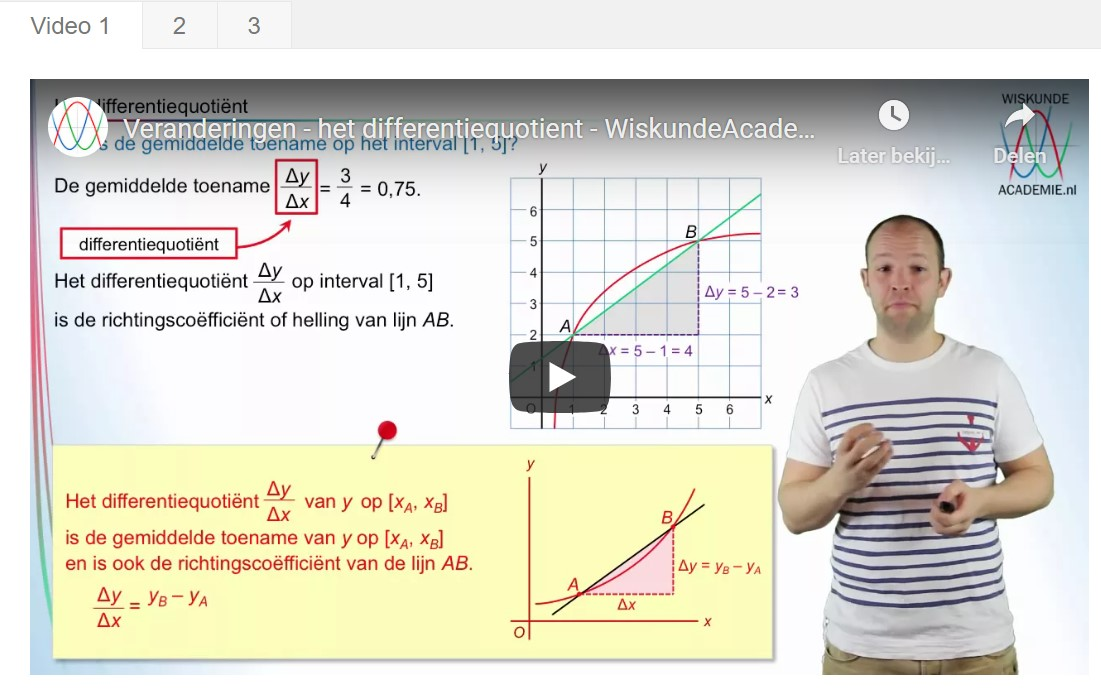
\includegraphics[width=\linewidth]{figurenAuteur/Schermafbeelding Wiskundeacademie.jpg}
\captionof{figure}{Schermafdruk Wiskundeacademie}
\end{center}\

De onderwerpen die aan bod komen zijn algebraïsche vaardigheden, exponentiële verbanden, combinatoriek, formules en functies, goniometrie, kansrekening, kwadratische verbanden, lineaire verbanden, meetkunde, machtsverbanden, statistiek, veranderingen en afgeleiden en vergelijkingen oplossen.

De onderwerpen zijn opgesplitst in meerdere korte video's. De video's kunnen dienen om geziene leerstof te herhalen, als leerlingen een les gemist hebben of om een nieuw begrip aan te brengen. 

\tussentitel{IntMath}

Op deze Engelstalige website kun je over veel verschillende onderwerpen een theoretische verklaring vinden. Je krijgt duidelijke voorbeelden waarbij ook het verband tussen wiskunde en de echte wereld getoond wordt. Met applets kan de gebruiker verschillende topics ontdekken en toepassen. De website is interactief en geeft uitleg bij de tussenstappen. Vermits alles gratis is, moet je de reclame tussen de opdrachten door erbij nemen.

Het feit dat deze website in het Engels is, biedt de mogelijkheid om niet zo taalvaardige leerlingen te laten ontdekken dat de taal geen probleem hoeft te zijn. Wiskunde is immers een universele taal: symbolen en formules zijn al hetzelfde en met de vertaling van enkele specifieke termen kom je al ver!  

Hieronder zie je een voorbeeldje uit de goniometrie over de formules van de dubbele hoek. 

\end{multicols}

\begin{center}
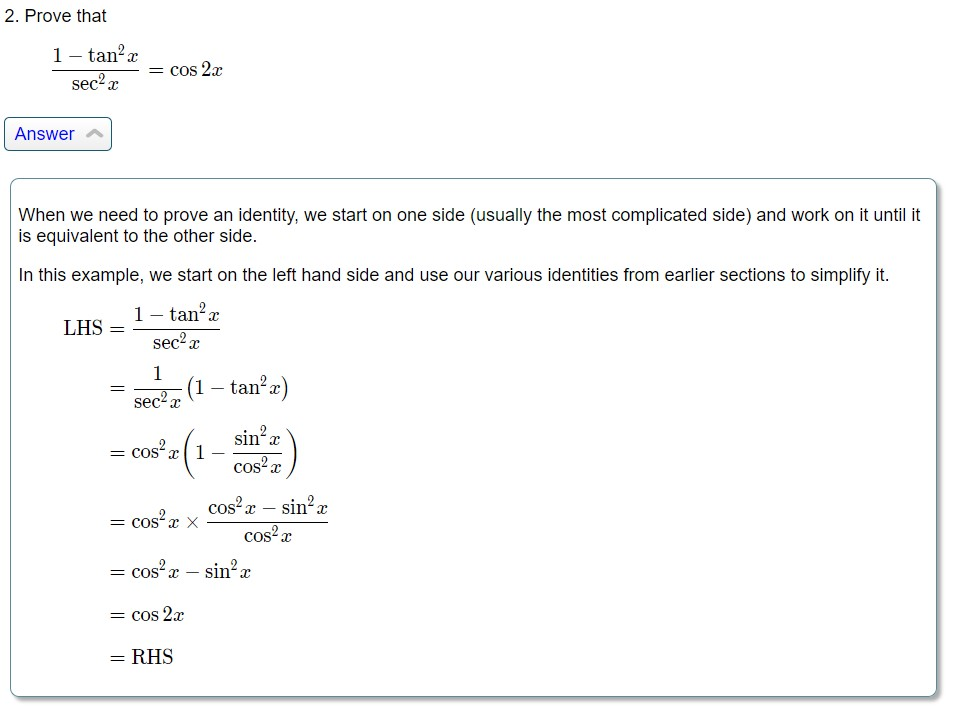
\includegraphics[width=11cm]{figurenAuteur/schermafdruk IntMath.jpg}
\captionof{figure}{Schermafdruk IntMath}
\end{center}
\begin{multicols} {2}


\tussentitel{Math4all}

Math4all zet zich in voor vernieuwing van wiskundig lesmateriaal. Deze website geeft uitleg en voorbeelden om leerlingen en leerkrachten te helpen bij het opzoeken en herhalen van kennis van andere (voorgaande) jaren. De website wil hulpmiddelen bieden voor versterking van `blended learning' met als basis een database die de mogelijkheid biedt tot het creëren van maatwerk.

AlgebraKIT is een onderdeel van deze website met de mogelijkheid om rekentechnieken in te oefenen. Hij beoordeelt tussenstappen en of leerlingen op de goede weg zitten. Deze methode geeft interactieve feedback, reeksen opgaven die automatisch gegenereerd worden en oefeningen voor leerlingen in elk stadium.

\begin{center}
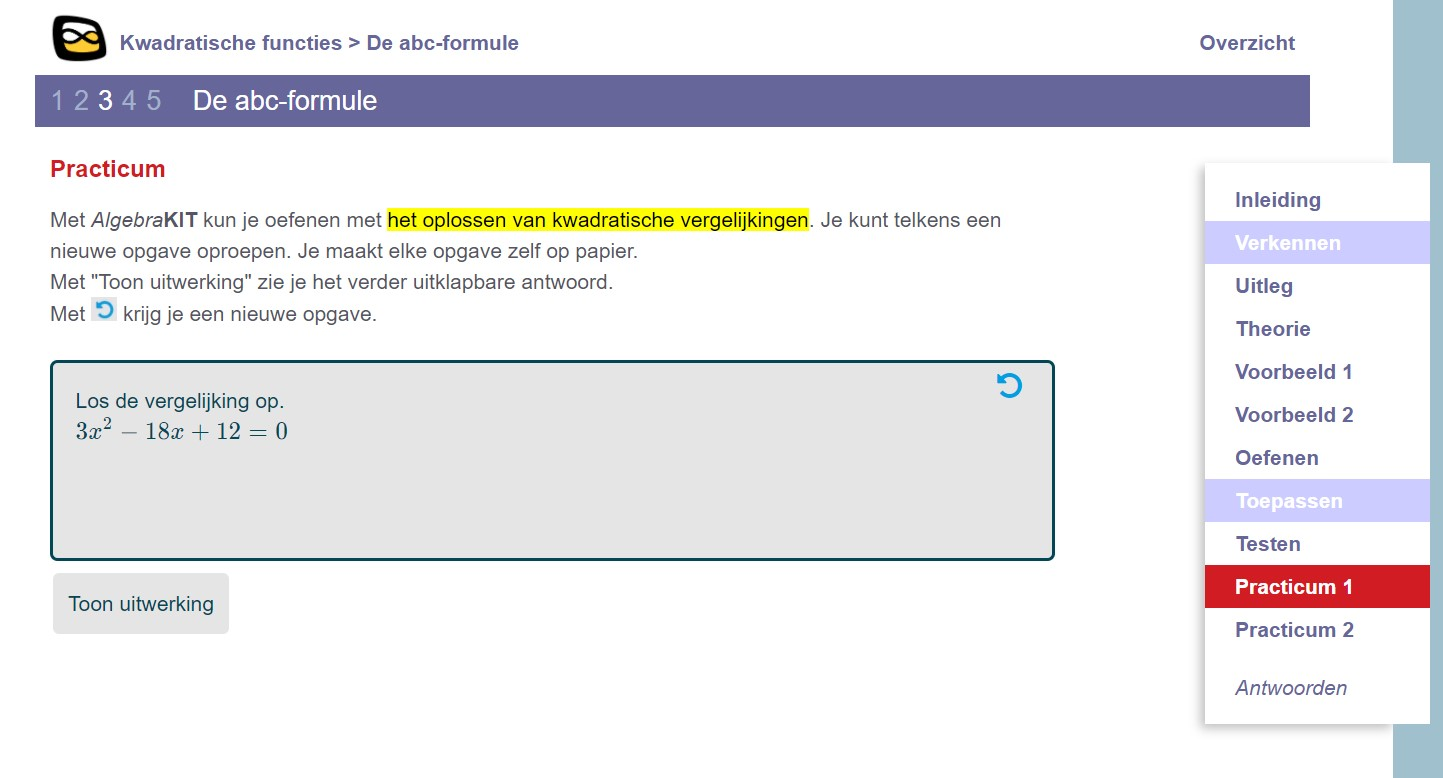
\includegraphics[width=\linewidth]{figurenAuteur/Schermafbeelding algebraKiT.jpg}
\captionof{figure}{Schermafdruk AlgebraKIT}
\end{center}

\tussentitel{YouTubekanaal patrickJMT}

Op deze website vind je filmpjes waarin Patrick heel veel wiskundebegrippen en onderwerpen uitlegt. Hij doceert alleen en legt verschillende rekentechnieken uit. Uiteraard nooit zo goed als de echte leraar, maar als je leraar niet binnen handbereik is, kun je er veel topics terugvinden. En Patrick doet het in het Engels.

\tussentitel{Usolv-it}

Hier vind je een heel groot aanbod multiplechoicevragen uit onder andere de Vlaamse Wiskunde Olympiades, de Kangoeroewedstrijden, ijkingstoetsen, toelatingsexamen voor arts en tandarts, oefeningen uit de handboekenreeks Van Basis tot Limiet...

Vooral handig aan deze site is dat je als leerkracht een toets of oefeningenreeks kunt samenstellen door vragen te filteren per onderwerp en niveau. Je kunt de vorderingen van je leerlingen opvolgen en linken aan Smartschool. 

Als leerkracht kun je gratis kennismaken gedurende twee weken. Een individueel lidmaatschap kost 50 EUR voor een jaar en een schoolabonnement voor 20 leerkrachten kost 100 EUR als je deelneemt aan de olympiades.

Leerlingen kunnen gratis en onbeperkt oefenen met een selectie oefeningen. Ze krijgen onmiddellijke feedback en vooral uitgeschreven oplossingen, niet alleen de einduitkomst. 

\begin{center}
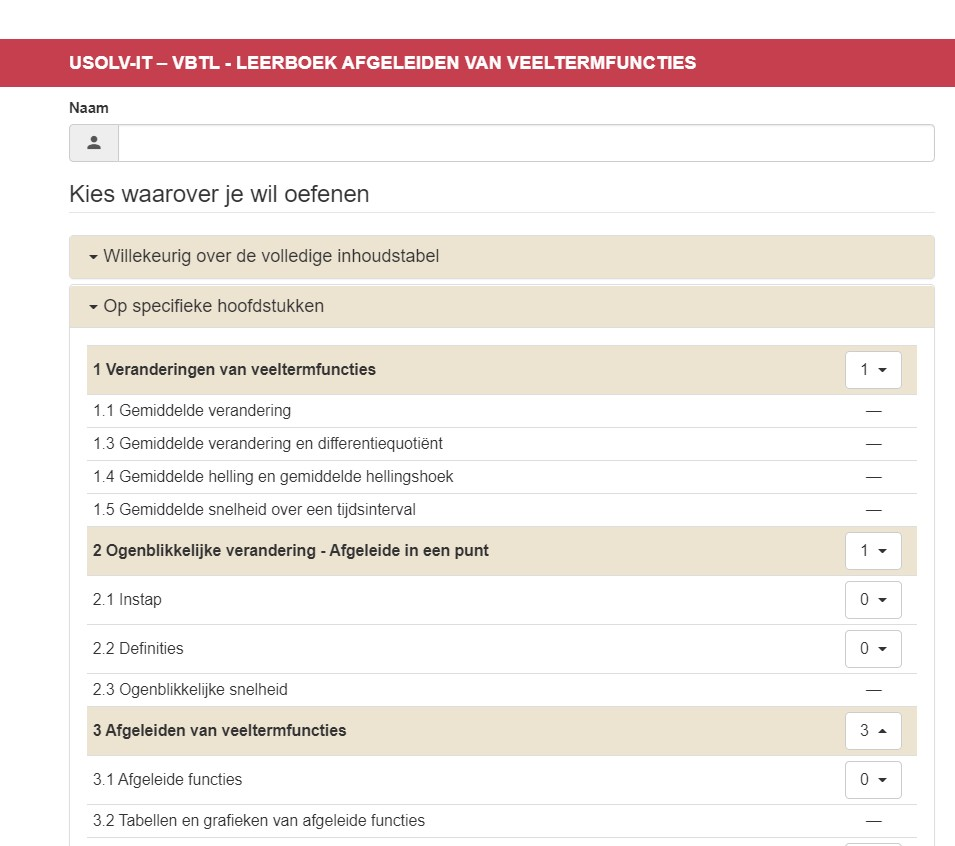
\includegraphics[width=\linewidth]{figurenAuteur/Schermafbeelding usolv-it.jpg}
\captionof{figure}{Schermafdruk Usolv-it}
\end{center}


\section{Tools voor noodgevallen}

We hebben allemaal onze weg moeten zoeken in het afstandsonderwijs, met vallen en opstaan. Door links en rechts rond te vragen hoe andere leraren problemen oplosten, heeft iedereen min of meer een eigen werkwijze gevonden. We zetten hier enkele nuttige tips op een rijtje die het allemaal wat haalbaarder maken. Het lijstje is opnieuw niet volledig. We delen wat we geleerd hebben... dat is tenslotte het doel van Uitwiskeling!

\tussentitel{Schoolafspraken en hergebruik van bestanden}

Wie had in maart gedacht dat alles zo lang ging duren? In mijn naïviteit heb ik mijn bestanden niet goed benoemd. Om materiaal optimaal te kunnen hergebruiken, is een goeie naamgeving en ordening van de bestanden essentieel.

De notities van de live-lessen gaf ik in het begin enkel de datum als bestandsnaam. Mijn lessen statistiek heb ik gewoon genummerd van 1 tot 10. Veel te laat ben ik begonnen met het lesonderwerp erbij te zetten en of het ging over notities van een live les, een ingesproken powerpoint, een filmpje. Sommige bestanden zoals bv. opnames van Google Meet worden automatisch ergens geplaatst waar je later geen zicht meer op hebt. Je computer op orde houden is altijd belangrijk, dat is nog maar eens gebleken. 

Ook goede afspraken op schoolniveau zijn broodnodig. 

Op de ene school deed iedereen de eerste weken maar wat hij of zij dacht dat goed was met als gevolg dat veel leerlingen door het bos de bomen niet meer zagen. Ze kregen opdrachten via berichten, via de digitale schoolagenda met bijlages, enz. Gaandeweg werden afspraken gemaakt: alle opdrachten mogen enkel nog opgegeven worden via de digitale schoolagenda en niet meer als bijlage van berichten. Alle digitale opdrachten moeten ingediend worden via de uploadzone van Smartschool met een vast sjabloon voor de naam van de bestanden: jjjjmmdd naam opdracht. Belangrijk voor de leerkracht is om goed na te denken over de structuur van de uploadzone.  

Op een andere school werd van in het begin met Google Classroom gewerkt. De structuur werd door de ICT-ondersteuners van de school en enkele ervaren leraren klaargezet voor iedereen. Dit werd door leerlingen en ouders erg gesmaakt. Ze kregen complimenten over de gestructureerde aanpak. 

Niet alle leerlingen waren van in het begin mee. Ook dit soort dingen moet aangeleerd worden. Dit schooljaar werd hierop geanticipeerd door dit goed op poten te zetten terwijl de leerlingen nog voltijds op school waren. 


\tussentitel{Gebruik van een tekentablet}
Vorig schooljaar heb ik bij het begin van de lockdown mijn uiterste best gedaan om zo goed mogelijk met mijn leerlingen te communiceren. Ik merkte al vlug dat ik praktisch niet goed genoeg uitgerust was en ook te weinig kennis had van wat er op de markt was. Ik had direct de behoefte om op de opdrachten van mijn leerlingen te kunnen schrijven zoals ik dat anders op papier zou doen. Ik had enkel een muis, maar dat was onmogelijk om daar iets meer dan een gerichte streep mee te trekken.

Ondertussen weet ik dat er tablets zijn die je kan neerleggen en waar je met een pen op kunt schrijven. Ik kon dat niet op mijn tablet. Ik kreeg de gouden tip om een tekentabletje aan te kopen. Deze bestaan in verschillende groottes met bijhorende prijskaartjes. Ik heb het kleinste model voor ongeveer 50 EUR aangekocht. Het tabletje is via een USB-kabeltje met mijn computer verbonden. Je schrijft er met de bijhorende pen op zoals op een blad papier. De hoekpunten zijn de referentiepunten van je scherm.

\begin{center}
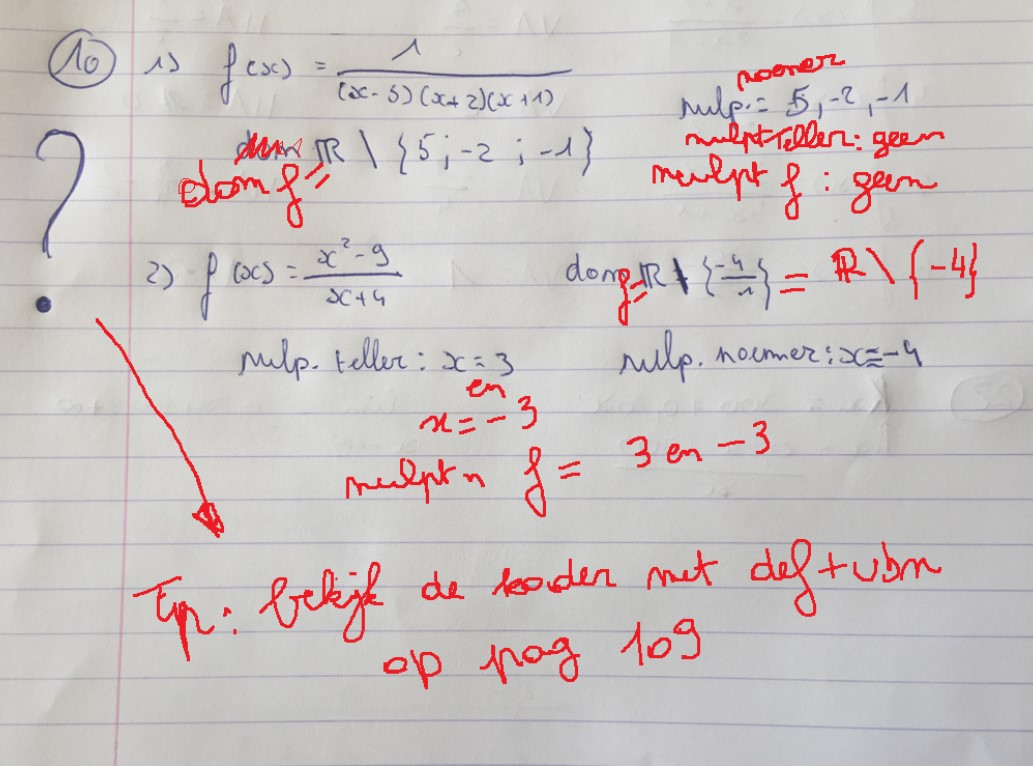
\includegraphics[width=\linewidth]{figurenAuteur/verbetering leerling.jpg}
\captionof{figure}{Met de pen en tekentablet verbeterd}
\end{center}

In het begin is het even wennen: je maakt met de pen  schrijfbewegingen op je (horizontaal) tekentabletje, maar je ziet enkel op je scherm waar en wat je schrijft. Het kleinste model volstaat voor wat ik er mee wil doen. Ik kan echt zeggen dat dit apparaatje me door de lockdown geholpen heeft... 

Ik heb deze tip ondertussen al vaak doorgegeven aan andere collega's. Mijn collega's technische vakken gebruiken nu ook een tabletje om tekeningen en ontwerpen na te kijken. Ze moeten tekeningen niet meer afprinten om ze na te kijken! 

\begin{center}
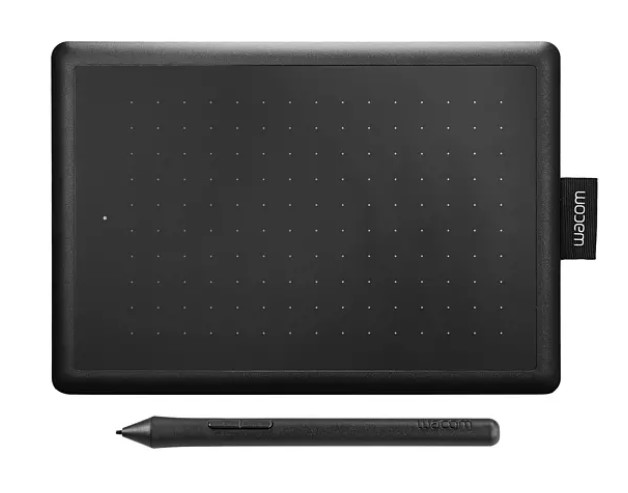
\includegraphics[width=\linewidth]{figurenAuteur/wacom.jpg}
\captionof{figure}{Tekentablet}
\end{center}

\tussentitel{OneNote-lessen}
Ik gebruikte mijn tekentablet ook om online live-les te geven met OneNote. Meestal zette ik een aantal oefeningen klaar en kon tijdens de les aantekeningen maken zoals ik dat op bord zou doen. Na de les bezorgde ik op vraag van de leerlingen mijn notities ook aan hen. Dan konden ze die nog eens herbekijken op eigen tempo.

\begin{center}
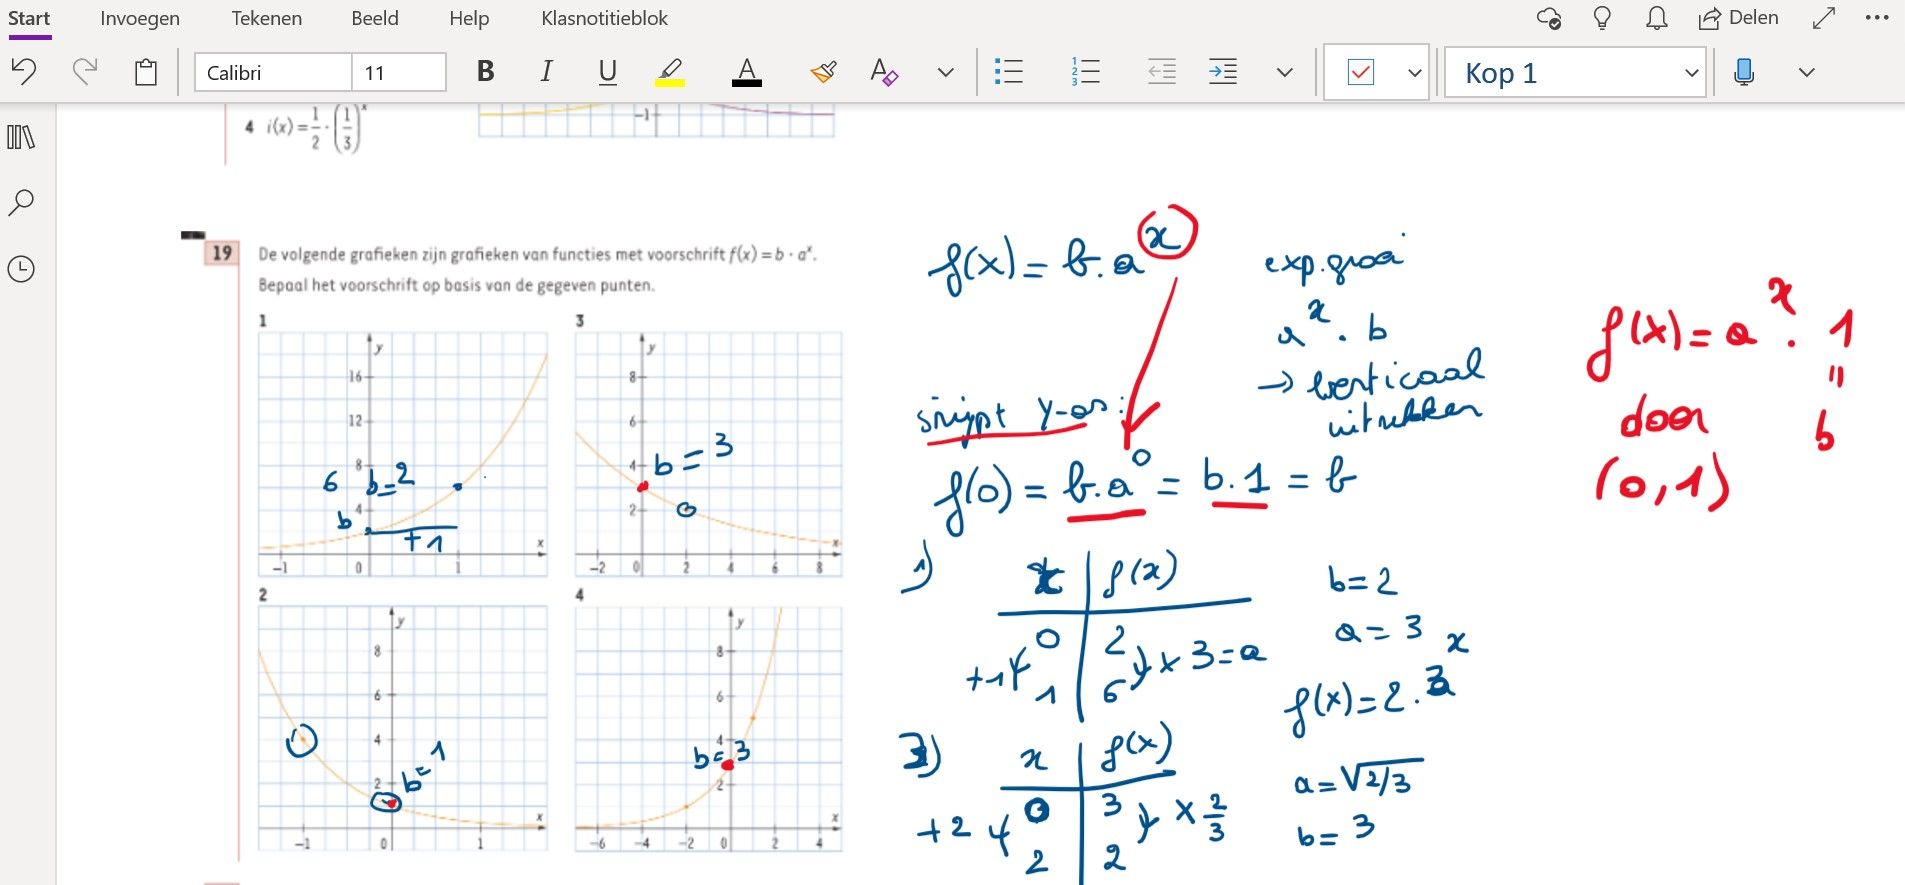
\includegraphics[width=\linewidth]{figurenAuteur/scherm onenote.jpg}
\captionof{figure}{OneNote met de tekenpen}
\end{center}

Dit kan ik ook toepassen bij gewoon onderwijs. Ik heb een digitaal bord in de klas en kan zo mijn bordnotities van de les opslaan en delen met leerlingen die wegens corona of een andere reden afwezig zijn. Een alternatief is uiteraard ook foto's trekken van je bordnotities en die doorgeven.
\vspace{0.5 cm}

\tussentitel{Bewerken van pdf}

In UW 36/04 beschreef ik al hoe leerlingen Office Lens kunnen gebruiken om met de hand geschreven documenten als één pdf-bestand te uploaden. Als leerkracht kun je dan weer met je tekentablet en pennetje dat bestand in één keer bewerken en terug uploaden. Ik gebruikte hiervoor het programma Foxit Reader. 

\begin{center}
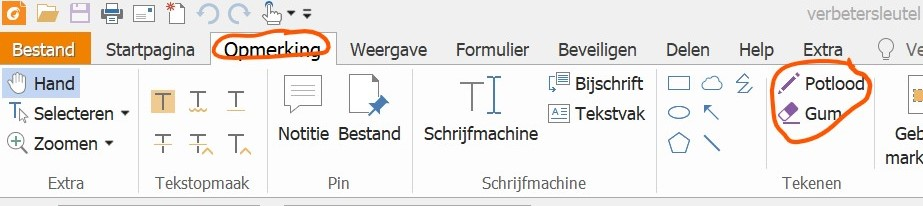
\includegraphics[width=\linewidth]{figurenAuteur/foxit pen.jpg}
\captionof{figure}{In het tabblad Opmerking vind je de tekentool}
\end{center}
\begin{center}
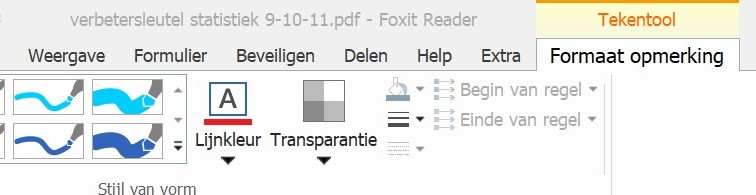
\includegraphics[width=\linewidth]{figurenAuteur/tekentool.jpg}
\captionof{figure}{Hier kun je de kleur en dikte van de pen instellen}
\end{center}

Een ander alternatief om op pdf-documenten te schrijven is drawboard PDF. Er zijn ook laptops of tablets waar een pen bijhoort waarmee je rechtstreeks op het scherm kunt schrijven. 

\tussentitel{Photomath}

Ik leerde deze tool jaren geleden kennen. Tijdens de lessen goniometrie in het vijfde jaar had ik gemerkt dat heel veel leerlingen moeite hadden met het rekenen met breuken. Als remediëringstaak gaf ik een lijstje met gemengde oefeningen op breuken zodat zij en ik konden zien welke rekenregels ze nog niet beheersten. Tot mijn grote verbazing hadden ze bijna allemaal alles juist. 

De leerlingen hadden Photomath ontdekt, een app op de smartphone die wiskundeoefeningen, getypt of handgeschreven, scant en oplost. Mijn doelstelling was helemaal onderuit gehaald maar dit voorval heb ik wel gebruikt om voortaan anders met taken om te gaan. Ik heb hen toen ook gevraagd om deze tool zinvol te gebruiken: niet enkel om een uitkomst te bekomen maar om zelf gemaakte oefeningen te controleren en tussenstappen te bekijken als ze vastzitten. 

De app is erg geëvolueerd sinds het begin. Hij kan uitdrukkingen uitwerken en vereenvoudigen, vergelijkingen en ongelijkheden oplossen, afgeleiden en integralen berekenen... De tussenstappen die getoond worden, komen niet altijd overeen met je eigen werkwijze. Maar je kunt de app zeker inzetten om je leerlingen zelf (standaard)oefeningen te laten controleren en je stapel verbeterwerk toch enigszins te verkleinen. Het blijft uiteraard nodig om deze rekenvaardigheden van je leerlingen zonder app te testen maar dan kun je je beperken tot een steekproef!  

\begin{center}
\includegraphics[width=0.6\linewidth]{figurenAuteur/photomath1.png}
\captionof{figure}{Photomath: de opgave met de oplossing}
\end{center}
\begin{center}
\includegraphics[width=0.6\linewidth]{figurenAuteur/Photomath2.png}
\captionof{figure}{Tussenstappen bij Photomath}
\end{center}

\tussentitel{Ingesproken powerpoint}

Als je beschikt over goede powerpoint-presen-taties, is er de mogelijkheid om die van geluid te voorzien en er nota's bij te maken. Het resultaat kunnen de leerlingen naar wens bekijken wanneer ze maar willen, zelfs meerdere keren als het nodig is. 

Deze methode was voor mij te tijdrovend omdat ik de presentaties zelf eerst nog moest maken. Eens gemaakt heb je deze dingen natuurlijk ook voor latere lessen. Je kunt uiteraard ook gewone powerpoints gebruiken om je onlinelessen te ondersteunen, en indien gewenst deze onlineles opnemen. 

\tussentitel{Zelf filmpjes maken}
Na een tip van een andere collega gebruikte ik  Screencast-O-Matic. Het is een eenvoudige onlinetool, bovendien gratis als je je beperkt tot 15 minuten durende filmpjes. Dat is eerder een voordeel dan een nadeel. Het dwingt me na te denken over wat ik zeker wil zeggen. Vijftien minuten naar een filmpje kijken is voor een leerling (en voor mij) lang genoeg. Je kunt kiezen of je zelf in beeld wil, je scherm wilt delen of een combinatie van beiden maken waar je jezelf onderaan rechts klein in beeld zet. Dit laatste zou zeer motiverend werken...

\begin{center}
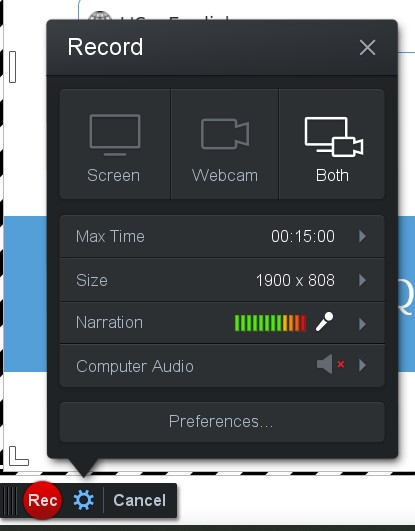
\includegraphics[width=\linewidth]{figurenAuteur/Screencastomatic knoppen.jpg}
\captionof{figure}{Instellingen van Screencast-O-Matic}\label{screencastomatic}
\end{center}

Zoals je kan zien in figuur \ref{screencastomatic} is het programma eenvoudig in gebruik met een beperkt aantal instructies.

\begin{center}
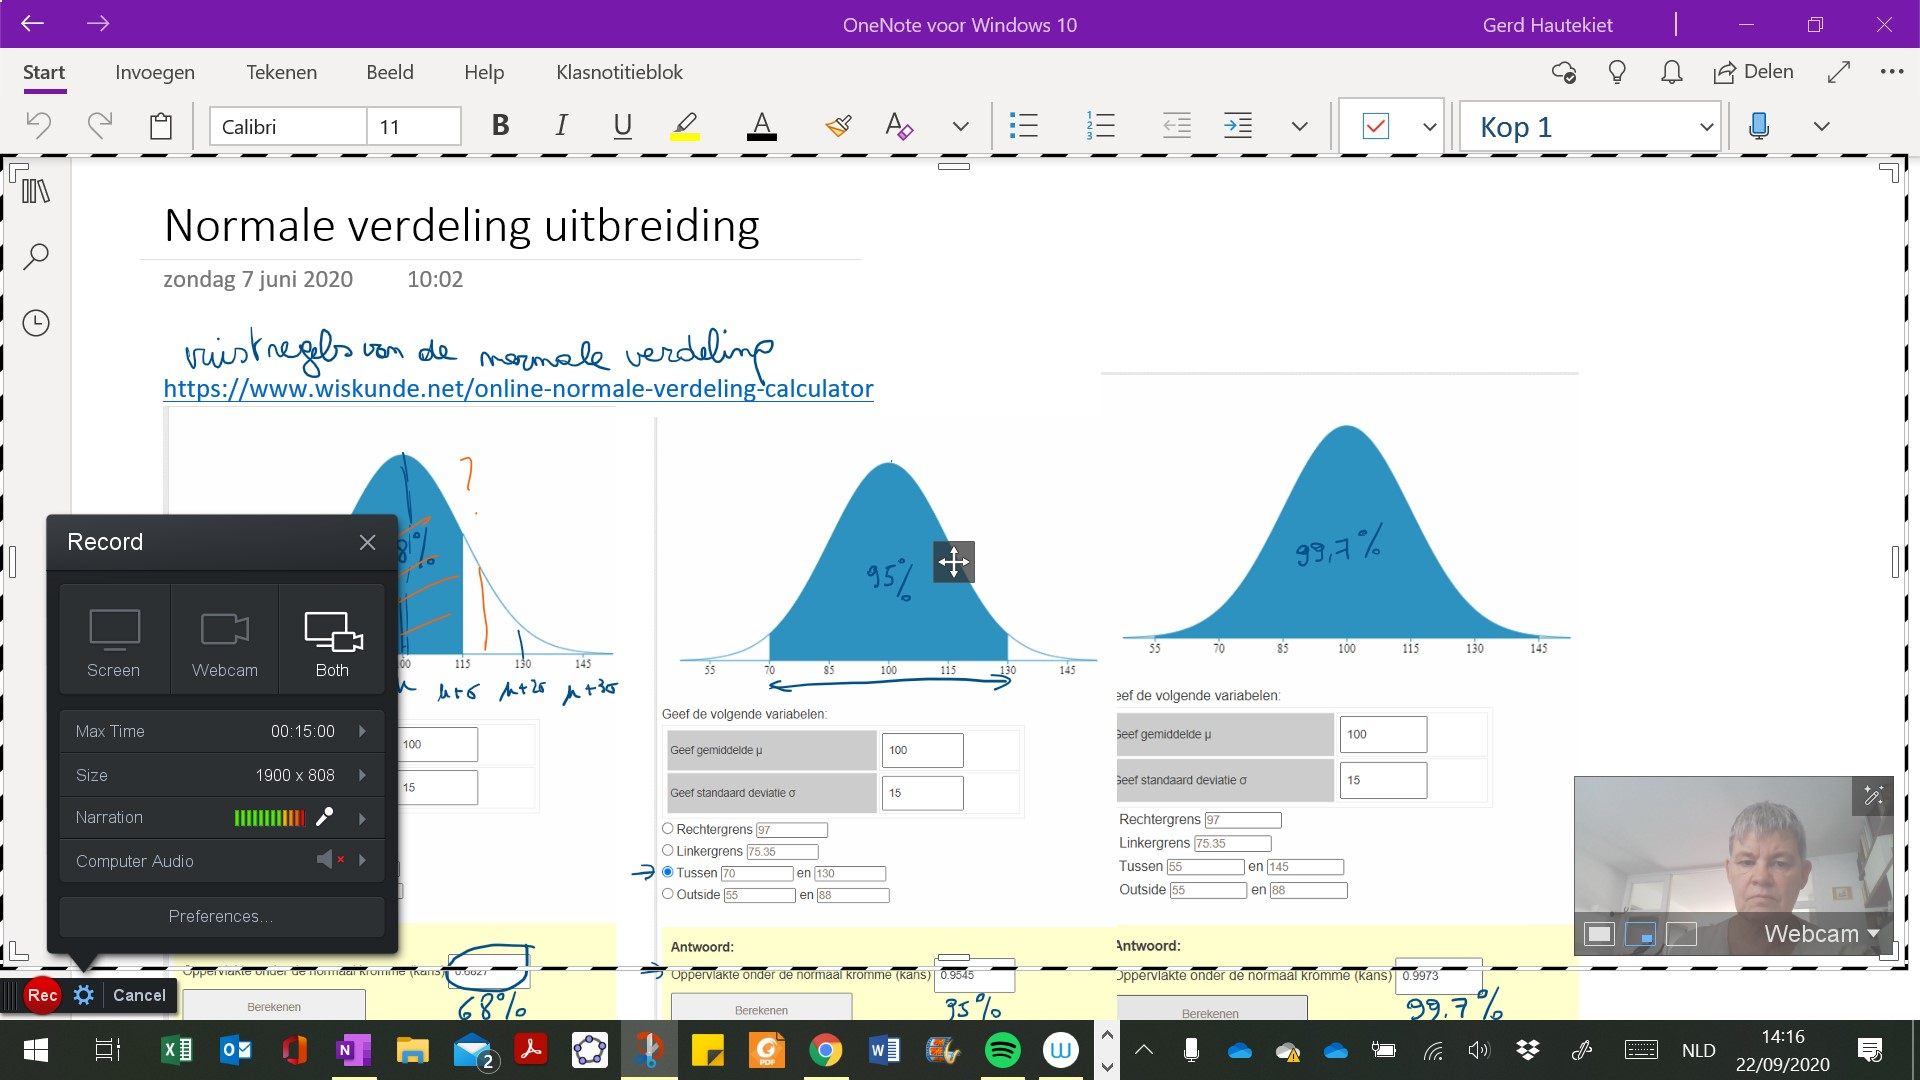
\includegraphics[width=\linewidth]{figurenAuteur/screenomatic.jpg}
\captionof{figure}{Schermafdruk van Screencast-O-Matic}\label{schermscreencastomatic}
\end{center}

Alles binnen de stippellijn wordt opgenomen (zie figuur \ref{schermscreencastomatic}). Je kunt de opname onderbreken en ondertussen van actief schermbeeld wisselen. Best zet je alles wat je nodig hebt voor je opname op voorhand klaar of open.  Op de website staan duidelijke korte tutorials. Handig want je wilt niet te veel tijd spenderen aan nieuwe tools, je wilt ze gewoon snel kunnen gebruiken. 

OBS (Open Broadcast Software) is een goed alternatief om filmpjes op te nemen. Maar omdat het meer mogelijkheden heeft, ligt de instapdrempel iets hoger. Maar OBS-gebruikers zijn over het algemeen ook enthousiast. Je kan OBS ook gebruiken om je lessen te streamen (zie verderop).

Ik gebruikte deze filmpjes voor verschillende doelen. Af en toe sprak ik mijn leerlingen toe om hen moed te geven, bij te sturen... met mezelf in beeld. Maar ik gebruikte de filmpjes vooral om een nieuw item eerst uit te leggen en daarna oefeningen op te geven. Daarbij gebruikte ik meestal OneNote waar ik al of niet stukken van het handboek, grafieken ... had klaargezet. Je kunt gemakkelijk onderbreken en de draad terug opnemen waar je de laatste keer gestopt bent. Zo moet je niet elke keer helemaal opnieuw beginnen als bijvoorbeeld de postbode aanbelt...

In het begin was ik zeer kritisch over mijn eigen filmpjes en begon ik dikwijls opnieuw. Ik was dan ook veel te lang bezig met één filmpje te maken. Naarmate het schooljaar vorderde was ik blij dat het er op stond en bekeek ik het eindresultaat zelfs niet opnieuw. Ook mijn leerlingen waren blij met deze filmpjes. Ze konden ze bekijken wanneer het hen uitkwam en zelfs meerdere keren als ze het nodig vonden. 

Deze filmpjes publiceer je best op een eigen YouTube-kanaal bijvoorbeeld. Met een code of een ingebedde link in Smartschool kunnen leerlingen de filmpjes herbekijken of terugspoelen zonder dat ze die moeten downloaden op hun eigen computer. Deze tool kun je later nog heel handig inzetten voor ´flipping the Classroom' of als je een les afwezig bent. 

\tussentitel{Opnemen of/en streamen van lessen}

De eenvoudigste methode is als je jezelf filmt terwijl je voor je bord of whiteboard staat (op school of thuis) en les geeft. Dit vraagt niet veel techniek. Zorg er wel voor dat de kwaliteit van het geluid goed genoeg is. De camera (smartphone) op een statief of driepikkeltje en een externe micro geven de beste opnamekwaliteit. 

Als de ene helft van je leerlingen thuis zit en de andere helft in de klas, kun je je les op dezelfde manier delen door Smartschool Live, Teams of Google Meet open te zetten en eventueel op te nemen. De afwezige leerlingen zullen misschien niet alles kunnen verstaan, niet alles kunnen lezen... maar ze zijn toch grotendeels bij de les en het klasgebeuren betrokken!

Wil je liever streamen via YouTube dan leggen we dat heel gedetailleerd uit op de website van Uitwiskeling. Dit heeft als voordeel dat leerlingen je les ook achteraf nog kunnen bekijken terwijl je geen echte opnames moet maken die veel geheugenruimte innemen op je computer. Ook dit kun je doen zonder professioneel materiaal. Een stabiel netwerk en internetverbinding zijn wel echt nodig. Verder volstaan een laptop, een smartphone op een driepikkel en streamingsoftware zoals OBS. Met behulp van OBS stream je je lessen naar een `streaming service provider' zoals YouTube. Daar moet je (minstens 24 uur op voorhand) een eigen YouTubekanaal aanmaken. Je leerlingen bekijken via een link dan je lessen op dat YouTubekanaal. Ook het scherm van je laptop kun je met een of meerdere vensters streamen. Het vraagt uiteraard wel wat oefening en uitproberen. Op internet vind je duidelijke tutorials om dit te fixen, bijvoorbeeld (Cottenier, 2020). 

\begin{center}
\includegraphics[width=\linewidth]{figurenAuteur/Streaming.png}
\captionof{figure}{Schermbeeld van een streaming}
\end{center}

\section{Nawoord}

Tot slot willen we opnieuw stilstaan bij het doel van deze loep. De lockdown was een periode waarin we veel nieuwe dingen uitprobeerden. Met dit artikel wilden we in kaart brengen hoe de kennis die we daarbij opdeden, ons onderwijs kan versterken. Daarbij benadrukken we opnieuw dat we geen voorstander van afstandsonderwijs zijn maar dat digitale elementen ons onderwijs wel kunnen ondersteunen. 

Tijdens de grote vakantie na de eerste lockdown, zijn we aan deze tekst beginnen schrijven. Op dat moment hoopten we om dit schooljaar voltijds voor de klas te staan. Ondertussen weten we dat het coronavirus nog niet weg was (en is). De situatie verandert voortdurend. Dit betekent dat we nog een hele tijd soepel en flexibel zullen moeten zijn. Wij en ook onze leerlingen leren nog steeds bij om met deze situatie om te gaan. We merken ook dat het aanbod van tools heel snel evolueert. Toch kozen we ervoor om dat wat we op dit moment kennen, te delen.

Als laatste element willen we nog meegeven dat de loep het resultaat is van een brainstorming met de hele redactie. We willen je zeker niet het gevoel geven dat je alles moet doen of gebruiken. We willen vooral inspireren en praktische hulp bieden. Als je door het lezen van deze loep al één gedachte, idee of oplossing kunt gebruiken, zijn wij geslaagd in onze opzet.

Zorg goed voor jezelf en de anderen! 

\end{multicols}
\vspace{1 cm}
% bronnen toevoegen
\begin{bronnen}
\item Cottenier Stefaan, \emph{Jouw lessen streamen met laptop en smartphone}
https://www.klascement.net/video/109563/jouw-lessen-streamen-met-laptop-en-smartphone/?previous
\item Kuhlemeier, H., Steentjes, M. (2002). \emph{Docenten wiskunde over open en meerkeuzevragen:
genuanceerder dan u denkt!}. Nieuwe Wiskrant 22-2/december 2002
\item Mason, J., Klymchuk, S. (2009). \emph{Using Counter-examples in Calculus}. Londen: Imperial College Press.
\item https://algebrakit-learning.com/
\item https://screencast-o-matic.com/
\item https://wiskundeacademie.nl/
\item https://www.intmath.com/
\item https://www.lerenzichtbaarmaken.nl/ 3/11/2020
\item patrickJMT youtube:https://www.youtube.com/channel/UCFe6jenM1Bc54qtBsIJGRZQ

\end{bronnen}

